\documentclass{unicam_thesis}
\usepackage[utf8]{inputenc}
\usepackage{listings}
\usepackage{braket}
\usepackage[backend=bibtex]{biblatex}
\usepackage[automake,toc,acronyms,nonumberlist, nopostdot]{glossaries}
\usepackage{mathabx}
\usepackage{amsthm}
\usepackage{graphicx} 
\usepackage{tikz}  
\usetikzlibrary{quantikz, positioning, arrows.meta, calc, automata, positioning, backgrounds, fit, shapes.geometric}
\usepackage{booktabs}     
\usepackage{subcaption}  
\usepackage{amsthm}
\usepackage{adjustbox}
\usepackage{amssymb}
\usepackage[utf8]{inputenc}
\usepackage[T1]{fontenc}
\usepackage{lmodern}
\usepackage[nottoc]{tocbibind}
\usepackage{hyperref}


\theoremstyle{plain}
\newtheorem{theorem}{Theorem}[section]
\newtheorem{lemma}{Lemma}[section]
\newtheorem{corollary}{Corollary}[section]
\newtheorem{proposition}{Proposition}[section]
\newtheorem{conjecture}{Conjecture}[section]
\newtheorem{assumption}{Assumption}[section]

\theoremstyle{definition}
\newtheorem{definition}{Definition}[section]
\newtheorem{example}{Example}[section]
\newtheorem{exercise}{Exercise}[section]
\newtheorem{algorithm}{Algorithm}[section]
\newtheorem{concept}{Concept}[section]

\theoremstyle{remark}
\newtheorem*{remark}{Remark}
\newtheorem{observation}{Observation}[section]
\newtheorem{notation}{Notation}[section]



\tikzset{rejecting/.style={circle, draw, red, dashed}}

\makeglossaries
\loadglsentries[acronym]{myglossaries}

\title{Systematic Taxonomy of Quantum Finite Automata: Bridging Classical and Quantum Computational Models}

\university{Universit\`a degli Studi di Camerino}
\school{Scienze e Tecnologie}
\course{Laurea in Informatica (Classe L-31)}


\author{Marta Musso}
\advisor{Relatore Name}
% add Marcello Bonsangue, Michele Loreti
\coadvisor2{Correlatore Name}
\academicyear{2024/2025}
\matricola{122360}

\graphicspath{{Screenshot/},{Pictures/},{API/},{Source/}}
\addbibresource{biblio.bib}
\begin{document}

\maketitle
\begin{abstract} {
    Quantum automata theory investigates how principles of quantum mechanics can be integrated with classical models of computation to reveal new limits and possibilities in computational power. Although the theory offers deep insights, progress has been slowed by inconsistent notation, unclear model definitions, and fragmented comparisons across different approaches. This thesis establishes a unified framework that standardises definitions and systematically compares classical finite automata with their quantum counterparts, focusing on state complexity and language recognition capabilities.

    The work begins with a comprehensive review of classical finite automata, including deterministic, nondeterministic, probabilistic, and two-way models, also specifying the formal language theory that underpins these models. This review lays the necessary theoretical foundation for the subsequent discussion of quantum finite automata.
    The thesis then introduces the foundational principles of quantum mechanics and explains how these underpin the definition of quantum automata. 
    Subsequently, the work reviews various quantum automata models, analyzing their formal definitions, computational dynamics and language recognition properties. 
    Lastly, the thesis presents a unified taxonomy that provides a systematic comparison between classical and quantum automata models, highlighting the computational capabilities and limitations of quantum automata.
    The unified framework presented here offers clear insights into the computational capabilities and limitations of quantum automata, and it provides a systematic basis for further research in quantum computational models.
}
\noindent\textbf{Keywords:} Quantum automata, finite automata taxonomy, computational complexity, hybrid quantum-classical models, formal language theory 
\end{abstract}
\newpage


\tableofcontents

%\lstlistoflistings
%\listoffigures
%\listoftables

\chapter{Introduction}  
\label{chap:introduction}

The intersection of quantum mechanics and theoretical computer science has given rise to quantum computing, a field that reimagines computational paradigms through the lens of quantum phenomena such as superposition, entanglement, and measurement. At its core lies quantum automata theory, which seeks to understand how these principles redefine the boundaries of classical computation. \glspl{cfa}—\gls{dfa}, \gls{nfa}, \gls{pfa}, and two-way variants—have long served as the bedrock of formal language theory, offering mathematically rigorous frameworks for analyzing computational complexity and decidability. In contrast, \glspl{qfa} exhibit probabilistic and non-deterministic behaviors that transcend classical limits, necessitating a coherent framework to classify and analyse their capabilities. This thesis emerges from the recognition that the current landscape of quantum automata theory is fragmented: definitions vary across papers, notations lack standardization, and comparisons between classical and quantum models remain scattered across disjointed works \cite{gruska2012quantum}. By systematically unifying these elements, this thesis aims to bridge the conceptual gap between classical and quantum computational models, offering a structured lens through which their interaction can be rigorously studied \cite{ambainis2009superiority}.  

The motivation for this work is two-fold: theoretical exploration and practical application. Theoretically, quantum automata represent the simplest quantum computational models, providing a sandbox to explore the interplay between quantum mechanics and computation. They challenge classical intuitions—for instance, quantum parallelism enables certain \glspl{qfa}, such as the \gls{mm-1qfa}, to recognise languages with exponentially fewer states than their classical counterparts \cite{ambainis1998one}. Practically, as quantum hardware advances, understanding the minimal resources required to implement \glspl{qfa} becomes critical for designing efficient algorithms and robust error-correcting schemes \cite{nielsen2010quantum}. Yet, progress in the field has been hindered by ambiguities in model definitions. For example, early quantum automata models like the \gls{mo-1qfa} and \gls{mm-1qfa} were defined with differing acceptance criteria, leading to confusion about their relative computational power \cite{kondacs1997power}. Similarly, hybrid models such as the \gls{1qfac} introduce classical memory components, complicating direct comparisons to purely quantum or classical automata \cite{li2012characterizations}. These inconsistencies obscure the true capabilities of quantum models and hinder cross-disciplinary collaboration.

A central observation motivating this thesis is that no single document currently catalogs quantum automata models alongside their classical counterparts. Existing surveys, while valuable, often focus on specific subsets of models or lack the granularity needed to resolve nuanced differences in computational power, closure properties, or decidability \cite{gruska2012quantum}. For instance, although the expressive power of \gls{2qfa} surpasses that of classical two-way automata, the conditions under which this advantage manifests—such as the role of quantum interference in recognizing non-regular languages—remain underexplored in a unified context \cite{yakaryilmaz2010succinctness}. Moreover, the literature review in this thesis is dedicated to clearly identifying the specific classes of languages each automaton model accepts. In contrast, this work adopts a taxonomic approach, dissecting each model’s formal definition, acceptance criteria, and operational dynamics while contextualizing its position within the broader hierarchy of automata. This approach not only clarifies existing results but also identifies gaps where further research is needed, such as the decidability of equivalence problems for \glspl{qfa} with mixed states or the precise trade-offs between quantum entanglement and space efficiency \cite{hirvensalo2012quantum}.  

The research challenges addressed in this thesis are multifaceted. First, reconciling disparate notation and definitions requires a meticulous synthesis of foundational and contemporary literature. For example, the transition from unitary operations in \gls{mo-1qfa} to superoperator-based transitions in open quantum systems, as seen in \glspl{otqfa}, calls for a unified formalism to compare their computational behaviors \cite{bertoni2001quantum, breuer2002theory}. Second, characterizing the relationships between classical and quantum models necessitates a framework that accounts for both their similarities (e.g., the ability of \gls{1qfac} to simulate \glspl{dfa}) and their divergences (e.g., the exponential state advantage of \gls{2qfa} over two-way probabilistic automata). Third, the absence of standardised pumping lemmas or minimization algorithms for \glspl{qfa} complicates efforts to classify their language recognition capabilities, a challenge that this thesis tackles through a comparative analysis of closure properties and equivalence criteria \cite{yakaryilmaz2014quantum}.  

To address these challenges, this thesis employs a structured methodology that unfolds in several stages. It begins by grounding the discussion in classical automata theory, revisiting \gls{dfa}, \gls{nfa}, \gls{pfa}, and two-way variants to establish foundational concepts. Building on this, the thesis introduces the foundational principles of quantum mechanics—such as superposition, entanglement, and measurement—which provide the basis for defining quantum finite automata \cite{nielsen2010quantum}. With this dual background in place, the work systematically explores various quantum models, ranging from early variants like the \gls{mo-1qfa} \cite{moore2000quantum} and the \gls{mm-1qfa} \cite{kondacs1997power} to advanced hybrids such as the \gls{1qfac} and enhanced models (e.g., the \gls{eqfa}). Each model is rigorously analysed along several dimensions: its formal definition is standardised, its acceptance criteria are scrutinised, and its computational dynamics—such as the role of measurement timing and the interplay between quantum and classical states—are carefully dissected, with particular emphasis on identifying the exact classes of formal languages recognised by each model.

A significant contribution of this work is the development of a hierarchical taxonomy of automata models, which organises both classical and quantum automata into a coherent structure based on their computational features and complexity classes. For example, the analysis reveals that \glspl{2qfa} occupy a higher complexity class than their one-way counterparts, while hybrid models such as the \gls{1qfac} serve as an intermediate bridge between purely quantum and purely classical models \cite{yakaryilmaz2010succinctness}. The taxonomy further highlights open research questions, such as the precise relationships between models that employ different quantum operational frameworks (e.g., \glspl{a-qfa} versus \glspl{gqfa}) and the conditions under which quantum automata outperform probabilistic models in language recognition tasks \cite{hirvensalo2012quantum}.

The thesis is organised to guide the reader through these progressively complex layers of analysis. Following this introduction, Chapter~\ref{chap:background} consolidates foundational concepts from both classical automata theory and quantum mechanics, providing a unified background for the discussions that follow. Chapter~\ref{chap:models} presents a comprehensive catalog of quantum automata models; each model is formally defined, its computational dynamics are analysed, and its language recognition capabilities are explicitly detailed. Chapter~\ref{chap:comparative-analysis} synthesises these findings by evaluating expressive power, closure properties, and decidability issues across different models. Finally, Chapter~\ref{chap:conclusion} concludes by reflecting on the thesis’s contributions and outlining directions for future research, such as solving open questions in equivalence checking for \glspl{qfa} \cite{li2012characterizations}, extending pumping lemmas to quantum models \cite{yakaryilmaz2014quantum}, and developing minimization algorithms for hybrid automata.

In essence, this thesis seeks to transform quantum automata theory from a collection of isolated results into a cohesive and systematic framework. By standardizing definitions, clarifying the relationships between different models, and identifying critical open challenges, the work provides both a valuable reference for researchers and a solid methodological basis for future advancements in quantum computational models. As quantum computing transitions from theory to practice, such systematic foundations will be essential for harnessing the full potential of quantum-enhanced computation.
\chapter{Background}  
\label{chap:background}

The study of quantum automata theory necessitates a thorough grounding in both classical computational models and the quantum mechanical principles that redefine their capabilities. This chapter systematically establishes the conceptual foundation for analyzing quantum automata by first revisiting classical finite automata—the cornerstone of formal language theory—and then introducing the quantum mechanical framework that underpins novel computational paradigms.

We begin with an in-depth exploration of classical finite automata, which serve as the theoretical bedrock for understanding computational limits and language recognition. \glspl{dfa}, \glspl{nfa}, \glspl{pfa}, and their two-way variants are analyzed through their formal definitions, operational dynamics, and closure properties. These models collectively define the boundaries of classical computation, particularly in recognizing regular languages and in delineating limitations when handling context-free or stochastic languages. Foundational works such as Hopcroft et al. \cite{hopcroft2006introduction}—which formalized the equivalence between \glspl{dfa} and \glspl{nfa}—and Rabin's seminal work on probabilistic automata \cite{rabin1963probabilistic} have played a pivotal role in shaping this understanding.

The discussion then transitions to the essential principles of quantum mechanics required for quantum computation. Key concepts such as qubit representation, quantum superposition, entanglement, and the measurement postulate are introduced and contextualized within computational frameworks. These principles fundamentally depart from classical bit-based processing by allowing phenomena such as state interference and probabilistic state collapse. The mathematical formalism provided by Nielsen and Chuang \cite{nielsen2010quantum} serves as the backbone for these quantum operations.

This chapter is organized to mirror the later hierarchical taxonomy of automata and sets the stage for analyzing hybrid models such as the \gls{1qfac} \cite{zheng2012one}, where classical memory is integrated with quantum processing, as well as for reviewing advanced quantum models.

\section{Classical Finite Automata}
\label{sec:classical-finite-automata} 

Finite automata form the cornerstone of formal language theory, providing mathematical frameworks to analyze computational limits and language recognition capabilities. This section systematically examines deterministic, nondeterministic, probabilistic, and two-way variants, emphasizing their structural relationships and computational boundaries. 

\subsection{Shared Foundations}
\label{subsec:shared-foundations}

The study of automata begins with foundational concepts in formal language theory, pioneered by figures such as Stephen Kleene \cite{kleene1956representation}, Noam Chomsky \cite{chomsky1956three}, Alan Turing \cite{hopcroft2006introduction}, and Michael Rabin \cite{rabin1963probabilistic}. Their seminal work established the mathematical scaffolding for analyzing computational models and laid the groundwork for both classical and modern computational theories. In this subsection, we elaborate on core definitions, fundamental operations, and language classifications, supplemented with practical examples, formal specifications, and key theoretical results.

\begin{notation}[Symbols]
In this thesis, the following notations are used:
\begin{itemize}
    \item $\Sigma$: an alphabet, i.e., a non-empty finite set of symbols.
    \item $\Sigma^\ast$: the Kleene closure of $\Sigma$, the set of all finite strings over $\Sigma$.
    \item $\epsilon$: the empty string (with $\|\epsilon\| = 0$).
    \item $\|w\|$: the length of a string $w$.
\end{itemize}
\end{notation}

\subsubsection{Alphabets and Strings}
An \textit{alphabet} $\Sigma$ is defined as a non-empty, finite set of symbols that serve as the basic elements for constructing strings and, consequently, languages. For instance:

\begin{example}
\textbf{Binary Alphabet:} $\Sigma = \{0, 1\}$ is central to digital computing and coding theory \cite{hopcroft2006introduction}.
\end{example}

\begin{example}
\textbf{ASCII Alphabet:} $\Sigma_{\text{ASCII}}$, which contains 128 distinct characters used for text encoding \cite{cady1986ascii}.
\end{example}

A \textit{string} (or \textit{word}) $w$ over $\Sigma$ is a finite sequence of symbols $a_1a_2\ldots a_n$, where each $a_i \in \Sigma$. The \textbf{length} of $w$, denoted by $\|w\|$, is defined as the total number of symbols in the string. The special string $\epsilon$, known as the \textbf{empty string}, has a length of zero ($\|\epsilon\| = 0$) \cite{hopcroft2006introduction}.

\begin{example}
For $\Sigma = \{a, b\}$, consider the string $w = aba$. Then, $\|w\| = 3$. Conversely, $w = \epsilon$ represents the absence of input.
\end{example}

\begin{remark}
The concepts of $\Sigma$, $\Sigma^\ast$, and $\epsilon$ form the foundation for all language constructions and are pivotal when defining operations such as concatenation and the Kleene star.
\end{remark}

In addition to defining strings, several operations are essential for manipulating them:
\begin{itemize}
    \item \textbf{Reversal}: The operation $w^R$ produces the string obtained by reversing the order of symbols in $w$ (e.g., $(abc)^R = cba$) \cite{hopcroft2006introduction}.
    \item \textbf{Substring}: A string $v$ is a substring of $w$ if there exist (possibly empty) strings $x$ and $y$ such that $w = xvy$ \cite{hopcroft2006introduction}.
\end{itemize}

\subsubsection{Languages and Operations}
A \textit{language} $L$ is a subset of $\Sigma^\ast$, where $\Sigma^\ast$ denotes the \textbf{Kleene closure} of $\Sigma$, defined as:
\[
\Sigma^\ast = \bigcup_{n=0}^\infty \Sigma^n, \quad \text{where } \Sigma^0 = \{\epsilon\}.
\]
\cite{kleene1956representation}

Languages are constructed and manipulated using various operations. These operations are central to proofs of language properties and decidability:

\begin{enumerate}
    \item \textbf{Concatenation}: For two languages $L_1$ and $L_2$, their concatenation is defined by 
    \[
    L_1 \cdot L_2 = \{xy \mid x \in L_1,\, y \in L_2\}.
    \]
    \begin{example}
    Let $L_1 = \{a, ab\}$ and $L_2 = \{b, ba\}$. Then,
    \[
    L_1 \cdot L_2 = \{ab, aba, abb, abba\},
    \]
    which demonstrates the formation of new languages by joining strings from different languages \cite{hopcroft2006introduction}.
    \end{example}

    \item \textbf{Union/Intersection}: These operations are defined as:
    \begin{align*}
        L_1 \cup L_2 &= \{w \mid w \in L_1 \text{ or } w \in L_2\}, \\
        L_1 \cap L_2 &= \{w \mid w \in L_1 \text{ and } w \in L_2\}.
    \end{align*}
    They allow the combination or filtering of languages based on shared elements \cite{hopcroft2006introduction}.

    \item \textbf{Kleene Star}: The Kleene star operation generates the set of all possible concatenations (including the empty string) of elements from a language:
    \[
    L^\ast = \bigcup_{i=0}^\infty L^i, \quad \text{where } L^i = \underbrace{L \cdot L \cdots L}_{i \text{ times}}.
    \]
    \begin{example}
    For $L = \{0, 1\}$, the set $L^\ast$ comprises all binary strings, including $\epsilon$ \cite{hopcroft2006introduction}.
    \end{example}

    \item \textbf{Complement}: The complement of a language $L$ with respect to $\Sigma^\ast$ is defined as 
    \[
    \overline{L} = \Sigma^\ast \setminus L.
    \]
    This operation is useful for expressing languages indirectly \cite{hopcroft2006introduction}.

    \item \textbf{Homomorphism}: A homomorphism is a function $h: \Sigma^\ast \to \Gamma^\ast$ that maps each symbol in $\Sigma$ to a string in $\Gamma^\ast$. For example, if $h(a) = 01$, then every occurrence of $a$ in a string is replaced by $01$ \cite{hopcroft2006introduction}.

    \item \textbf{Inverse Homomorphism}: Given a homomorphism $h$, the inverse homomorphism is defined by 
    \[
    h^{-1}(L) = \{w \mid h(w) \in L\},
    \]
    which retrieves the pre-images from the target language \cite{hopcroft2006introduction}.
\end{enumerate}

\subsubsection{Language Categories}
Languages are classified according to the type of automata that recognize them and their inherent structural complexity. The main categories are as follows:

\begin{enumerate}
    \item \textbf{\glspl{dfa} and \glspl{nfa}}:  
    These languages are recognized by \gls{dfa} and \gls{nfa} and can be generated by regular expressions \cite{hopcroft2006introduction}. 
    \begin{example}
    $L = \{w \in \{a, b\}^\ast \mid w \text{ contains } aba\}$ is a regular language \cite{hopcroft2006introduction}.
    \end{example}
    
    \item \textbf{\glspl{pda}}:  
    These languages are recognized by \gls{pda} and generated by context-free grammars \cite{chomsky1956three, hopcroft2006introduction}.  
    \begin{example}
    $L_{\text{pal}} = \{ww^R \mid w \in \{a, b\}^\ast\}$, the language of palindromes, is a classic example \cite{chomsky1956three}.
    \end{example}

    \item \textbf{Context-Sensitive Languages}:  
    Recognized by linear-bounded automata, these languages have structural constraints that extend beyond context-free languages \cite{chomsky1956three, hopcroft2006introduction}.  
    \begin{example}
    $L = \{a^n b^n c^n \mid n \geq 1\}$ is an example of a context-sensitive language \cite{chomsky1956three}.
    \end{example}

    \item \textbf{Recursively Enumerable Languages (Type-0)}:  
    Recognized by \glspl{tm}, these languages embody the notion of algorithmic computability \cite{hopcroft2006introduction, turing1936computable}.  
    \begin{example}
    The language corresponding to the Halting Problem is recursively enumerable \cite{hopcroft2006introduction}.
    \end{example}

    \item \textbf{Stochastic Languages}:  
    Recognized by \glspl{pfa} with bounded error, stochastic languages allow for probabilistic acceptance criteria \cite{rabin1963probabilistic}.  
    \begin{example}
    $L_{\text{eq}} = \{a^n b^n \mid n \geq 1\}$ is stochastic but not regular. A \gls{pfa} can accept it with probability at least $\frac{2}{3}$ for strings in $L_{\text{eq}}$ and at most $\frac{1}{3}$ for strings not in $L_{\text{eq}}$ \cite{rabin1963probabilistic}.
    \end{example}
\end{enumerate}

\begin{definition}[Regular Language]
A language $L \subseteq \Sigma^\ast$ is \textit{regular} if there exists a \gls{dfa} (or an equivalent \gls{nfa}) that accepts exactly the strings in $L$.
\end{definition}

\begin{theorem}[Pumping Lemma for Regular Languages]
\label{thm:pumping-lemma}
Let $L \subseteq \Sigma^\ast$ be a regular language. Then there exists an integer $p \geq 1$, known as the \textit{pumping length}, such that every string $s \in L$ with $\|s\| \geq p$ can be decomposed into three parts $s = xyz$, satisfying:
\begin{enumerate}
    \item $|xy| \leq p$,
    \item $|y| \geq 1$, and
    \item For all $i \geq 0$, the string $xy^iz \in L$.
\end{enumerate}
\end{theorem}

\begin{corollary}
If a language $L$ fails to satisfy the conditions of Theorem~\ref{thm:pumping-lemma} for any possible pumping length $p$, then $L$ is not regular.
\end{corollary}

\subsubsection{Closure Properties}
Closure properties determine how language classes behave under various operations—a critical aspect in proving decidability and constructing new languages:

\begin{itemize}
    \item \textbf{\glspl{dfa} and \glspl{nfa}}: Regular languages are closed under union, intersection, complement, concatenation, and Kleene star \cite{hopcroft2006introduction}.
    \item \textbf{\glspl{pda}}: Context-free languages are closed under union and Kleene star, but not under intersection or complement \cite{chomsky1956three, hopcroft2006introduction}.
    \item \textbf{Context-Sensitive Languages}: Context-sensitive languages are closed under union, intersection, and complement \cite{chomsky1956three, hopcroft2006introduction}.
    \item \textbf{Stochastic Languages}: Stochastic languages are closed under union, intersection, and concatenation, but not under complementation or Kleene star \cite{rabin1963probabilistic, paz1971introduction}.
\end{itemize}

\begin{observation}
Closure properties not only simplify the construction of new languages from known ones but also play a key role in proving undecidability results. For instance, the non-closure of context-free languages under intersection and complementation is a cornerstone in many undecidability proofs.
\end{observation}

\begin{example}
The closure of regular languages under intersection guarantees that if $L_1, L_2 \in \glspl{dfa}$ (or, equivalently, recognized by \glspl{nfa}) then $L_1 \cap L_2$ is also regular. In contrast, although stochastic languages are closed under intersection, they are not closed under complementation, as demonstrated by the inability to recognize 
\[
\overline{L_{\text{eq}}} \quad \text{for} \quad L_{\text{eq}} = \{a^n b^n \mid n \geq 1\}
\]
\cite{rabin1963probabilistic}.
\end{example}

\begin{table}[h]
    \centering
    \begin{adjustbox}{max width=\textwidth}
    \begin{tabular}{@{}lccccc@{}}
        \toprule
        \textbf{Operation} & \glspl{dfa} & \glspl{pda} & Context-Sensitive & Stochastic & Type-0 \\ \midrule
        Union          & \checkmark & \checkmark & \checkmark & \checkmark & \checkmark \\
        Intersection   & \checkmark & $\times$ & \checkmark & \checkmark & \checkmark \\
        Complement     & \checkmark & $\times$ & \checkmark & $\times$ & \checkmark \\
        Concatenation  & \checkmark & \checkmark & \checkmark & \checkmark & \checkmark \\
        Kleene Star    & \checkmark & \checkmark & \checkmark & $\times$ & \checkmark \\ \bottomrule
    \end{tabular}
    \end{adjustbox}
    \caption{Comparison of closure properties for different language classes}
    \label{tab:closure-properties}
\end{table}

\subsubsection{Chomsky Hierarchy}
Formal languages are organized into a hierarchical framework known as the Chomsky hierarchy \cite{chomsky1956three, hopcroft2006introduction}:
\begin{enumerate}
    \item \textbf{Type-3 (Regular)}: Languages recognized by \glspl{dfa} (or \glspl{nfa}) \cite{hopcroft2006introduction}.
    \item \textbf{Type-2 (Context-Free)}: Languages recognized by \gls{pda} \cite{chomsky1956three}.
    \item \textbf{Type-1 (Context-Sensitive)}: Languages recognized by linear-bounded automata \cite{chomsky1956three}.
    \item \textbf{Type-0 (Recursively Enumerable)}: Languages recognized by Turing machines (\gls{tm}), which formalize the notion of algorithmic computability \cite{hopcroft2006introduction, turing1936computable}.
\end{enumerate}

\begin{concept}
The Chomsky hierarchy not only classifies languages based on the computational power needed for recognition but also reflects the trade-offs between expressiveness and computational complexity.
\end{concept}

\begin{figure}[h]
    \centering
    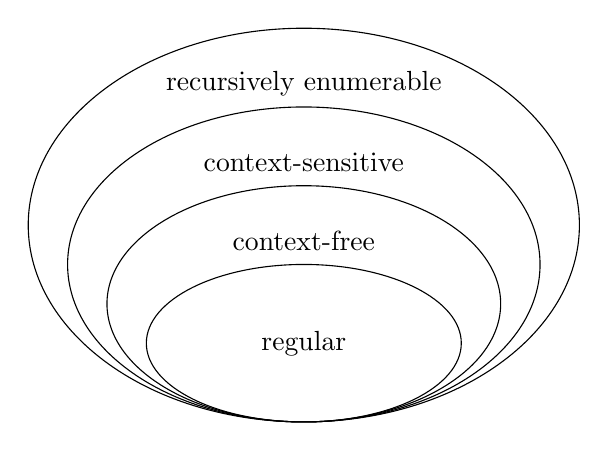
\begin{tikzpicture}
        \draw (0,0) ellipse (2 and 1);
        \draw (0,0.5) ellipse (2.5 and 1.5);
        \draw (0,1) ellipse (3 and 2);
        \draw (0,1.5) ellipse (3.5 and 2.5);
        \node at (0,0) {regular};
        \node at (0,1.3) {context-free};
        \node at (0,2.3) {context-sensitive};
        \node at (0,3.3) {recursively enumerable};
    \end{tikzpicture}
    \caption{Chomsky hierarchy of formal languages}
    \label{fig:chomsky-hierarchy}
\end{figure}

\subsubsection{Practical Implications}
The theoretical constructs discussed above are not only of academic interest but also have significant practical applications:
\begin{itemize}
    \item \textbf{Regular Expressions}: Extensively used in text processing (e.g., in tools such as \texttt{grep} and in lexical analyzers) \cite{kernighan1984unix, hopcroft2006introduction}.
    \item \textbf{Context-Free Grammars}: Form the basis for defining the syntax of programming languages such as Python and Java \cite{chomsky1956three, hopcroft2006introduction}.
    \item \textbf{Closure Properties}: Provide a framework for proving decidability results (e.g., the emptiness problem for \glspl{dfa}) \cite{hopcroft2006introduction}.
    \item \textbf{Stochastic Models}: Are applied in areas like natural language processing and speech recognition, where probabilistic pattern matching is essential \cite{rabin1963probabilistic}.
\end{itemize}

\subsubsection{Automata Definition Fundamentals}
All automata share several core structural components that provide the basis for their computational behavior \cite{hopcroft2006introduction, chomsky1956three}.

\begin{definition}[Classical Finite Automaton]
\label{def:finite-automaton}
A \textit{finite automaton} is a computational model that processes input symbols to recognize languages. Formally, a finite automaton $M$ is a quintuple $(Q, \Sigma, \delta, q_0, F)$, where:
\begin{itemize}
    \item \textbf{States ($Q$)}: A finite set of configurations representing the progress of computation \cite{hopcroft2006introduction}.
    \item \textbf{Input Alphabet ($\Sigma$)}: A finite set of symbols that the automaton processes \cite{hopcroft2006introduction}.
    \item \textbf{Transition Function ($\delta$)}: A function that governs state changes based on input. For deterministic models, $\delta: Q \times \Sigma \to Q$ (i.e., a \gls{dfa}); for nondeterministic models, $\delta: Q \times \Sigma \to 2^Q$ (i.e., an \gls{nfa}) \cite{chomsky1956three, hopcroft2006introduction}.
    \item \textbf{Initial State ($q_0 \in Q$)}: The starting configuration of the automaton \cite{hopcroft2006introduction}.
    \item \textbf{Accept States ($F \subseteq Q$)}: A subset of states that, when reached, indicate successful recognition of an input string \cite{hopcroft2006introduction}.
\end{itemize}
\end{definition}

\begin{remark}
The quintuple $(Q, \Sigma, \delta, q_0, F)$ is a standard representation that facilitates uniform analysis across different classes of automata.
\end{remark}

\begin{example}
The \gls{dfa} in Figure~\ref{fig:dfa-example} is defined by:
\begin{itemize}
    \item $Q = \{q_0, q_1\}$,
    \item $\Sigma = \{0, 1\}$,
    \item Transitions such as $\delta(q_0, 1) = q_1$ and $\delta(q_1, 0) = q_0$ (partial specification),
    \item $F = \{q_1\}$, indicating that the automaton accepts strings with an even number of 1s.
\end{itemize}
\end{example}

\begin{observation}
Graphical representations—using states, transitions, and designated initial/accept states—provide an intuitive understanding of automata behavior that complements the formal definitions.
\end{observation}

Graphical notation typically includes:
\begin{itemize}
    \item \textbf{States}: Represented by circles labeled with $q_i$.
    \item \textbf{Initial state}: Indicated by an incoming arrow (e.g., pointing to $q_0$).
    \item \textbf{Accept states}: Denoted by double circles (e.g., $q_1$ in Figure~\ref{fig:dfa-example}).
    \item \textbf{Transitions}: Illustrated by directed edges with labels representing input symbols.
\end{itemize}

\begin{table}[htbp]
    \centering
    \begin{adjustbox}{max width=\textwidth}
      \begin{tabular}{@{}lllll@{}}
          \toprule
          \textbf{Automaton} & \textbf{State Memory} & \textbf{Transition Type} & \textbf{Acceptance Condition} \\ \midrule
          \gls{dfa} & None & Deterministic & Final state membership \cite{hopcroft2006introduction} \\
          \gls{nfa} & None & Nondeterministic & Existence of an accepting path \cite{hopcroft2006introduction} \\
          \gls{pda} & Stack & Deterministic/Nondeterministic & Final state and empty stack \cite{chomsky1956three} \\
          \gls{tm} & Tape & Deterministic & Halting in an accept state \cite{turing1936computable} \\
          \bottomrule
      \end{tabular}
    \end{adjustbox}
    \caption{Automata representation variations}
    \label{tab:automata-variations}
\end{table}

\subsection{Deterministic Finite Automata (DFA)}
\label{subsec:dfa} 

As a specialization of the general finite automaton framework~\ref{def:finite-automaton} established in Section~\ref{subsec:shared-foundations}, a Deterministic Finite Automaton (DFA)\cite{hopcroft2006introduction} is formally defined as a quintuple \( M = (Q, \Sigma, \delta, q_0, F) \) where:
\begin{itemize}
    \item \( Q \): Finite set of states
    \item \( \Sigma \): Finite input alphabet
    \item \( \delta: Q \times \Sigma \rightarrow Q \): Total transition function
    \item \( q_0 \in Q \): Unique initial state
    \item \( F \subseteq Q \): Set of accepting states
\end{itemize}

\subsubsection{Language Recognition and Expressive Power}
DFAs precisely characterize the class of regular languages (\(\mathsf{REG}\)) within the Chomsky hierarchy \cite{hopcroft2006introduction}. Key properties include:

\begin{enumerate}
    \item \textbf{Closure Properties}: Closed under union, intersection, complement, concatenation, and Kleene star \cite{myhill1957finite}.
    \item \textbf{Limitations}: Cannot recognize non-regular languages like \( \{a^nb^n | n \geq 0\} \) (pumping lemma consequence) \cite{sipser2012introduction}.
    \item \textbf{Equivalence}: All regular expressions have corresponding DFAs and vice versa (Kleene's theorem) \cite{kleene1956representation}.
\end{enumerate}

The Myhill-Nerode theorem provides a canonical minimal DFA for any regular language, establishing state minimality criteria \cite{nerode1958linear}.

\subsubsection{Graphical Representation}
Consider the DFA in Figure~\ref{fig:dfa-example} recognizing strings with an even number of \texttt{0}s and \texttt{1}s. The automaton transitions between states based on input symbols, accepting strings that satisfy the parity constraints.

\begin{figure}[h]
    \centering  
    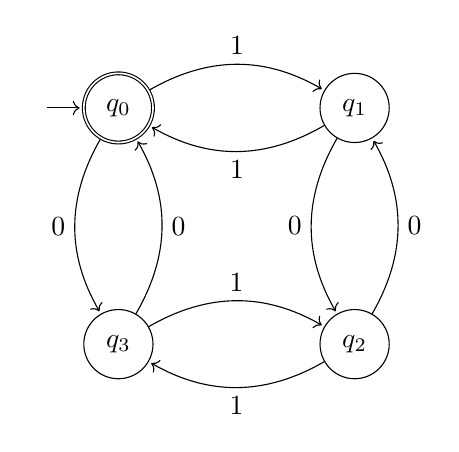
\begin{tikzpicture}[shorten >=1pt, node distance=3cm, on grid, auto]
        \node[state, initial, accepting, initial text={}] (q0) {$q_0$};
        \node[state] (q1) [right=of q0] {$q_1$};
        \node[state] (q2) [below=of q1] {$q_2$};
        \node[state] (q3) [left=of q2] {$q_3$};

        \path[->]
        (q0) edge [bend left] node {1} (q1)
        (q0) edge [bend right] node[swap] {0} (q3)
        (q1) edge [bend right] node[swap] {0} (q2)
        (q1) edge [bend left] node {1} (q0)
        (q2) edge [bend left] node {1} (q3)
        (q2) edge [bend right] node[swap] {0} (q1)
        (q3) edge [bend right] node[swap] {0} (q0)
        (q3) edge [bend left] node {1} (q2);
    \end{tikzpicture}
    \caption{DFA recognizing even numbers of \texttt{0}s and \texttt{1}s.}
    \label{fig:dfa-example}
\end{figure}

\(
L = \{ w \in \{0, 1\}^* \mid \text{the number of } 0\text{'s in } w \text{ is even and the number of } 1\text{'s in } w \text{ is even} \}
\) is the language recognized by this DFA.

The DFA is deterministic because for each state and input symbol (either \texttt{0} or \texttt{1}), there is exactly one transition defined. This ensures that from any given state, the next state is uniquely determined by the current input symbol, leaving no ambiguity in the automaton's behavior.

The structure of the DFA ensures that it keeps track of the parity (even or odd) of the counts of \texttt{0}s and \texttt{1}s as it processes each input symbol, transitioning between states accordingly to accept only those strings that meet the specified criteria.


\subsection{\acrfull{nfa}}
\label{subsec:nfa}

\begin{definition}[\gls{nfa}]
A \gls{nfa} is a quintuple 
\[
M = (Q, \Sigma, \delta, q_0, F)
\]
where:
\begin{itemize}
    \item \( Q \) is a finite set of states,
    \item \( \Sigma \) is an input alphabet,
    \item \( \delta: Q \times (\Sigma \cup \{\epsilon\}) \rightarrow 2^Q \) is a nondeterministic transition function,
    \item \( q_0 \in Q \) is the initial state, and
    \item \( F \subseteq Q \) is the set of accepting states.
\end{itemize}
\end{definition}

\begin{remark}
Unlike \glspl{dfa}, a \gls{nfa} may have multiple transitions for a given state and input symbol, including transitions on the empty string \(\epsilon\). This nondeterminism allows for multiple computational paths.
\end{remark}

\begin{example}
Figure~\ref{fig:nfa-example} depicts a \gls{nfa} that recognises the language 
\[
L = \{ w \in \{a,b\}^* \mid w \text{ contains the substring } ab \}.
\]
\end{example}

\begin{algorithm}[Subset Construction for \glspl{nfa}]
\label{alg:subset}
To convert an \gls{nfa} \( N = (Q, \Sigma, \delta, q_0, F) \) into an equivalent \gls{dfa}:
\begin{enumerate}
    \item Compute the \(\epsilon\)-closure of the initial state: \( S_0 = \epsilon\text{-closure}(\{q_0\}) \).
    \item For each \gls{dfa} state \( S \subseteq Q \) and each input symbol \(\sigma \in \Sigma\), define 
    \[
    \delta_{\text{\gls{dfa}}}(S, \sigma) = \epsilon\text{-closure}\Big(\bigcup_{q \in S} \delta(q, \sigma)\Big).
    \]
    \item Mark \( S \) as accepting if \( S \cap F \neq \emptyset \).
    \item Repeat until no new states are produced.
\end{enumerate}
\end{algorithm}

\begin{observation}
The subset construction algorithm may produce up to \(2^{|Q|}\) states in the worst case, illustrating a potential state explosion when converting an \gls{nfa} to a \gls{dfa}.
\end{observation}

\begin{figure}[h]
    \centering  
    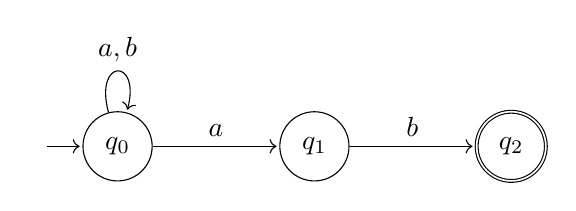
\begin{tikzpicture}[shorten >=1pt, node distance=2.5cm, on grid, auto]
        \node[state, initial, initial text={}] (q0) {$q_0$};
        \node[state] (q1) [right=of q0] {$q_1$};
        \node[state, accepting] (q2) [right=of q1] {$q_2$};

        \path[->]
        (q0) edge [loop above] node {$a,b$} (q0)
        (q0) edge node {$a$} (q1)
        (q1) edge node {$b$} (q2);
    \end{tikzpicture}
    \caption{NFA recognizing \( L = \Sigma^*ab \)}
    \label{fig:nfa-example}
\end{figure}

\begin{figure}[h]
    \centering  
    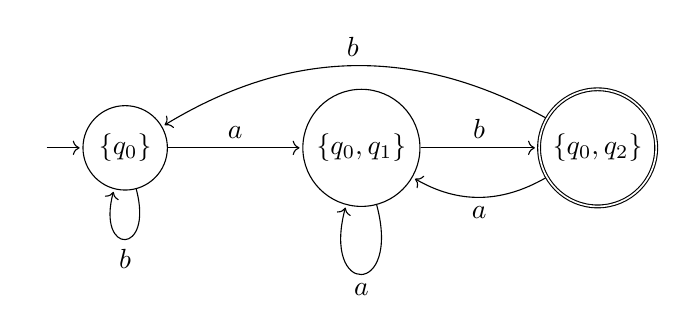
\begin{tikzpicture}[shorten >=1pt, node distance=3cm, on grid, auto]
        \node[state, initial, initial text={}] (A) {$\{q_0\}$};
        \node[state] (B) [right=of A] {$\{q_0, q_1\}$};
        \node[state, accepting] (C) [right=of B] {$\{q_0, q_2\}$};

        \path[->]
        (A) edge [loop below] node {$b$} (A)
        (A) edge node {$a$} (B)
        (B) edge [loop below] node {$a$} (B)
        (B) edge node {$b$} (C)
        (C) edge [bend left] node {$a$} (B)
        (C) edge [bend right] node[swap] {$b$} (A);
    \end{tikzpicture}
    \caption{Equivalent DFA for NFA in Figure~\ref{fig:nfa-example} \cite{hopcroft2006introduction}}
    \label{fig:dfa-conversion}
\end{figure}
\subsection{Probabilistic Finite Automata (PFA)}
\label{subsec:pfa}

As a generalization of the classical finite automaton framework~\ref{def:finite-automaton} established in Section~\ref{subsec:shared-foundations}, a Probabilistic Finite Automaton (PFA)\cite{rabin1963probabilistic} is formally defined as a quintuple \( M = (Q, \Sigma, \delta, \pi, F) \) where:
\begin{itemize}
    \item \( Q \): Finite set of states
    \item \( \Sigma \): Finite input alphabet
    \item \( \delta: Q \times \Sigma \times Q \rightarrow [0,1] \): Probabilistic transition function satisfying \( \sum_{q' \in Q} \delta(q, \sigma, q') = 1 \) for all \( q \in Q \), \( \sigma \in \Sigma \)
    \item \( \pi \in \mathbb{R}^{|Q|} \): Initial state distribution vector with \( \sum_{q \in Q} \pi_q = 1 \)
    \item \( F \subseteq Q \): Set of accepting states
\end{itemize}

\subsubsection{Language Recognition and Expressive Power}
PFAs recognize stochastic languages through probabilistic acceptance criteria. The language recognized by a PFA \( M \) with cut-point \( \lambda \in [0,1) \) is:
\[ L(M, \lambda) = \{ w \in \Sigma^* \mid \Pr[M \text{ accepts } w] > \lambda \} \]

Key variants and their properties include:

\begin{enumerate}
    \item \textbf{Isolated Cut-Point (\( \lambda \) with margin \( \epsilon > 0 \))}:
    \[ \Pr[M \text{ accepts } w] \begin{cases} 
    \geq \lambda + \epsilon & \text{if } w \in L \\
    \leq \lambda - \epsilon & \text{if } w \notin L 
    \end{cases} \]
    Recognizes exactly the regular languages \cite{rabin1963probabilistic}
    
    \item \textbf{Non-Isolated Cut-Point (\( \lambda = 0 \))}:
    \[ L(M, 0) = \{ w \mid \Pr[M \text{ accepts } w] > 0 \} \]
    Recognizes languages beyond regular, including context-sensitive \cite{paz1971introduction}
    
    \item \textbf{Strict Cut-Point (\( \lambda = 1 \))}:
    \[ L(M, 1) = \{ w \mid \Pr[M \text{ accepts } w] = 1 \} \]
    Equivalent to deterministic finite automata \cite{salomaa1969probabilistic}
\end{enumerate}

\subsubsection{Closure Properties}
PFAs exhibit nuanced closure characteristics compared to classical models:
\begin{itemize}
    \item Closed under union, intersection, and reversal \cite{paz1971introduction}
    \item \textbf{Not closed} under complementation unless using isolated cut-points \cite{bertoni1994closure}
    \item Kleene star closure requires additional constraints on transition probabilities \cite{hromkovic2000probabilistic}
\end{itemize}

\subsubsection{Graphical Representation}
Consider a PFA recognizing \( L_{\text{maj}} = \{ w \in \{a,b\}^* \mid |w|_a > |w|_b \} \) with probability \( \geq 2/3 \):

\begin{figure}[h]
    \centering  
    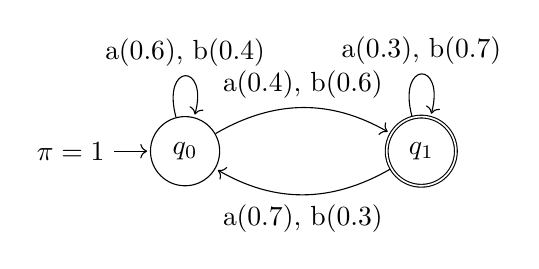
\begin{tikzpicture}[shorten >=1pt, node distance=3cm, on grid, auto]
        \node[state, initial, initial text={$\pi=1$}] (q0) {$q_0$};
        \node[state, accepting] (q1) [right=of q0] {$q_1$};
        
        \path[->]
        (q0) edge [loop above] node {a(0.6), b(0.4)} (q0)
        (q0) edge [bend left] node {a(0.4), b(0.6)} (q1)
        (q1) edge [loop above] node {a(0.3), b(0.7)} (q1)
        (q1) edge [bend left] node {a(0.7), b(0.3)} (q0);
    \end{tikzpicture}
    \caption{PFA for majority language with probabilistic transitions}
    \label{fig:pfa-example}
\end{figure}

This PFA maintains a probability distribution across states, with transitions weighted by input symbol probabilities. Acceptance occurs when the cumulative probability in \( F \) exceeds the cut-point after processing the entire input.

\subsubsection{Key Theoretical Results}
\begin{enumerate}
    \item \textbf{Rabin's Theorem}: PFAs with isolated cut-points recognize exactly \(\mathsf{REG}\) \cite{rabin1963probabilistic}
    \item \textbf{Pumping Lemma}: Probabilistic version requires probability bounds on loop iterations \cite{paz1971introduction}
    \item \textbf{Equivalence Problem}: Undecidable for PFAs with non-isolated cut-points \cite{tzelepis2021undecidable}
\end{enumerate}
%%%%%%%%%%%%%%%%%%%%%%%%%%%%%%%%%%%%%%%%%%%%%%%%%%%%%%%%%%%%%%%
% Two-Way Finite Automata Variants
%%%%%%%%%%%%%%%%%%%%%%%%%%%%%%%%%%%%%%%%%%%%%%%%%%%%%%%%%%%%%%%

\subsection{Two-Way Finite Automata Variants}
\label{subsec:two-way-variants}

Two-way finite automata extend the classical one‐way model by allowing the read head to move in both directions over the input. Although this extra power does not increase the class of recognizable languages (both one‐way and two‐way automata recognize exactly the regular languages), two‐way models can be exponentially more succinct than one‐way models and naturally lend themselves to algorithms in several contexts (e.g., in complexity analysis and even quantum models).

%%%%%%%%%%%%%%%%%%%%%%%%%%%%%%%%%%%%%%%%%%%%%%%%%%%%%%%%%%%%%%%
% Two-Way Deterministic Finite Automata (2DFA)
%%%%%%%%%%%%%%%%%%%%%%%%%%%%%%%%%%%%%%%%%%%%%%%%%%%%%%%%%%%%%%%

\subsubsection{\acrfull{2dfa}}
\label{subsubsec:2dfa}

\begin{definition}[Two-Way Deterministic Finite Automaton]
A \gls{2dfa} is formally defined as an 8-tuple 
\[
M = (Q, \Sigma, L, R, \delta, s, t, r),
\]
where:
\begin{itemize}
  \item \(Q\) is a finite set of states,
  \item \(\Sigma\) is a finite input alphabet,
  \item \(L\) and \(R\) are special symbols called the left and right endmarkers, respectively (with \(L,R \notin \Sigma\)),
  \item \(\delta: Q \times (\Sigma \cup \{L, R\}) \to Q \times \{L, R\}\) is the transition function,
  \item \(s\in Q\) is the start state,
  \item \(t\in Q\) is the (unique) accept state, and
  \item \(r\in Q\) (with \(r\neq t\)) is the (unique) reject state.
\end{itemize}
In addition, the transition function is assumed to satisfy:
\begin{itemize}
  \item For every state \(q\in Q\), when reading the left endmarker \(L\), the head always moves to the right; that is, \(\delta(q,L) = (q', R)\) for some \(q'\in Q\).
  \item Similarly, when reading the right endmarker \(R\), the head always moves to the left: \(\delta(q,R) = (q', L)\).
  \item Once the machine reaches the accept state \(t\) (or the reject state \(r\)), it remains there (the transition always maps back to itself) while moving in a fixed direction.
\end{itemize}
\end{definition}

\begin{remark}
The two-way motion allows the automaton to perform multiple passes over the input, which can result in an exponential reduction in the number of states compared to one-way automata, though at the expense of increased operational complexity.
\end{remark}

\begin{example}[First and Last Symbol Equality]
Consider the language 
\[
L = \{ w\in \{0,1\}^* \mid \text{the first symbol of } w \text{ equals the last symbol} \}.
\]
A \gls{2dfa} for \(L\) operates as follows:
\begin{enumerate}
  \item Start at the left endmarker \(L\) and immediately move right to read the first symbol; store it in the control.
  \item Continue scanning right until the right endmarker \(R\) is reached.
  \item Upon reading \(R\), reverse direction (move left) and, in the process, skip any blank moves until the last symbol is reached.
  \item Compare the stored first symbol with the last symbol. If they are equal, move to the accept state \(t\); otherwise, move to the reject state \(r\).
\end{enumerate}
A simplified state diagram illustrating this process is provided in Figure~\ref{fig:2dfa-example}.
\end{example}

\begin{observation}
Although every \gls{2dfa} can be simulated by a one-way \gls{dfa}, such a simulation may require an exponential increase in the number of states.
\end{observation}

\paragraph{Operational Mechanics}
The two-way motion enables the automaton to make multiple passes over the input, which is particularly useful for verifying properties that depend on both the prefix and the suffix of the input string.

\paragraph{State Complexity and Conversion Algorithms}
For some families of regular languages, \glspl{2dfa} can be exponentially more succinct than their one-way counterparts. Conversion algorithms—such as those proposed by Shepherdson and Kozen—use crossing sequences to simulate two-way behavior in a one-way \gls{dfa}, typically at the cost of exponential state blow-up.

%%%%%%%%%%%%%%%%%%%%%%%%%%%%%%%%%%%%%%%%%%%%%%%%%%%%%%%%%%%%%%%
% Two-Way Nondeterministic Finite Automata (2NFA)
%%%%%%%%%%%%%%%%%%%%%%%%%%%%%%%%%%%%%%%%%%%%%%%%%%%%%%%%%%%%%%%

\subsubsection{\acrfull{2nfa}}
\label{subsubsec:2nfa}

\begin{definition}[Two-Way Nondeterministic Finite Automaton]
A \gls{2nfa} is defined similarly to a \gls{2dfa} but with a nondeterministic transition function. Formally, a \gls{2nfa} is an 8-tuple
\[
M = (Q, \Sigma, L, R, \delta, s, t, r),
\]
where:
\begin{itemize}
    \item \(Q\) is a finite set of states,
    \item \(\Sigma\) is a finite input alphabet,
    \item \(L\) and \(R\) are the left and right endmarkers (with \(L,R\notin\Sigma\)),
    \item \(\delta: Q \times (\Sigma \cup \{L,R\}) \to 2^{\,Q \times \{L,R\}}\) is the nondeterministic transition function,
    \item \(s\in Q\) is the start state,
    \item \(t\in Q\) is the unique accept state, and
    \item \(r\in Q\) (with \(r\neq t\)) is the unique reject state.
\end{itemize}
The transition function obeys similar boundary conditions as in the \gls{2dfa} case.
\end{definition}

\begin{remark}
The nondeterminism in a \gls{2nfa} allows it to "guess" important positions within the input and verify them via bidirectional traversal, which can lead to significant state savings compared to deterministic models.
\end{remark}

\begin{example}[Symmetry Check (Toy Version)]
Consider the language 
\[
L_{sym} = \{ w \in \{0,1\}^* \mid \text{the first two symbols equal the last two symbols} \}.
\]
A high-level description of a \gls{2nfa} for \(L_{sym}\) is:
\begin{enumerate}
    \item Scan right from the left endmarker \(L\) while nondeterministically guessing the point where comparison will occur.
    \item Upon reaching the right endmarker \(R\), reverse direction.
    \item While moving left, nondeterministically check that the stored first two symbols match the corresponding symbols at the end.
    \item If both comparisons succeed, transition to the accept state \(t\); otherwise, transition to the reject state \(r\).
\end{enumerate}
Figure~\ref{fig:2nfa-example} schematically illustrates this guess-and-check mechanism.
\end{example}

\begin{observation}
\glspl{2nfa} can be exponentially more succinct than one-way \glspl{dfa}, even though the class of languages they recognize remains the same (i.e., the regular languages).
\end{observation}

%%%%%%%%%%%%%%%%%%%%%%%%%%%%%%%%%%%%%%%%%%%%%%%%%%%%%%%%%%%%%%%
% Two-Way Probabilistic Finite Automata (2PFA)
%%%%%%%%%%%%%%%%%%%%%%%%%%%%%%%%%%%%%%%%%%%%%%%%%%%%%%%%%%%%%%%

\subsubsection{\acrfull{2pfa}}
\label{subsubsec:2pfa}

\begin{definition}[Two-Way Probabilistic Finite Automaton]
A \gls{2pfa} is an 8-tuple
\[
M = (Q, \Sigma, L, R, \delta, s, t, r),
\]
where:
\begin{itemize}
    \item \(Q\) is a finite set of states,
    \item \(\Sigma\) is a finite input alphabet,
    \item \(L\) and \(R\) are the left and right endmarkers (with \(L,R \notin \Sigma\)),
    \item \(\delta: Q \times (\Sigma \cup \{L,R\}) \to \mathbb{R}_{\ge 0}^{\,Q \times \{L,R\}}\) is a probabilistic transition function such that
    \[
    \sum_{(q',d)\in Q\times\{L,R\}} \delta(q,a,q',d) = 1 \quad \text{for all } q \in Q \text{ and } a \in \Sigma \cup \{L,R\},
    \]
    \item \(s\in Q\) is the start state,
    \item \(t\in Q\) is the unique accept state, and
    \item \(r\in Q\) (with \(r\neq t\)) is the unique reject state.
\end{itemize}
\end{definition}

\begin{remark}
A \gls{2pfa} extends the probabilistic finite automaton by allowing bidirectional head movement. Its transitions are governed by probability distributions, and acceptance is determined by whether the cumulative probability of reaching the accept state exceeds a predetermined cut-point.
\end{remark}

\begin{example}[Majority Language]
Consider the language 
\[
L_{maj} = \{ w \in \{a,b\}^* \mid \#a(w) > \#b(w) \}.
\]
A \gls{2pfa} for \(L_{maj}\) operates by making probabilistic passes over the input, updating state probabilities, and eventually halting in the accept state \(t\) if the acceptance probability is high enough. Figure~\ref{fig:2pfa-example} provides a schematic illustration of such a machine.
\end{example}

\begin{theorem}[Rabin's Theorem for \glspl{pfa}]
\label{thm:2pfa-rabin}
A \gls{pfa} with an isolated cut-point recognizes exactly the class of regular languages. This result extends to \glspl{2pfa} under analogous conditions.
\end{theorem}

\begin{proposition}
If a \gls{2pfa} employs a non-isolated cut-point (e.g., \(\lambda = 0\)), it may recognize languages beyond the regular class.
\end{proposition}

\begin{corollary}
For a \gls{2pfa} with a strict cut-point (\(\lambda = 1\)), the recognized language is equivalent to that of a \gls{dfa}.
\end{corollary}

%%%%%%%%%%%%%%%%%%%%%%%%%%%%%%%%%%%%%%%%%%%%%%%%%%%%%%%%%%%%%%%
% Comparative Analysis of Two-Way Models
%%%%%%%%%%%%%%%%%%%%%%%%%%%%%%%%%%%%%%%%%%%%%%%%%%%%%%%%%%%%%%%

\subsubsection{Comparative Analysis of Two-Way Models}
\label{subsubsec:two-way-comparison}

\begin{table}[h]
    \centering
    \begin{adjustbox}{max width=\textwidth}
    \begin{tabular}{|l|c|c|c|c|l|}
        \hline
        \textbf{Model} & \textbf{Language Class} & \textbf{Time Complexity} & \textbf{Space Complexity} & \textbf{State Complexity} & \textbf{Key Reference} \\
        \hline
        \gls{2dfa}  & REG & \(O(n^2)\) & \(O(1)\) & May be exponentially smaller than 1DFA & \cite{hopcroft2006introduction} \\
        \gls{2nfa}  & REG & \(O(n)\) & \(O(1)\) & Can be exponentially more succinct than 1DFA & \cite{yakaryilmaz2010succinctness} \\
        \gls{2pfa}  & \( \mbox{REG} \subset L \subseteq \mbox{P} \) & \(O(n^3)\) & \(O(\log n)\) & Varies with error bounds & \cite{freivalds1981probabilistic} \\
        \hline
    \end{tabular}
    \end{adjustbox}
    \caption{Comparison of classical two-way automata models (using explicit endmarkers).}
    \label{tab:two-way-comparison}
\end{table}

\begin{remark}
The comparative analysis illustrates that while all two-way automata recognize only regular languages, the two-way models often achieve significant advantages in state complexity and, in some cases, time complexity, compared to their one-way counterparts.
\end{remark}

\begin{center}
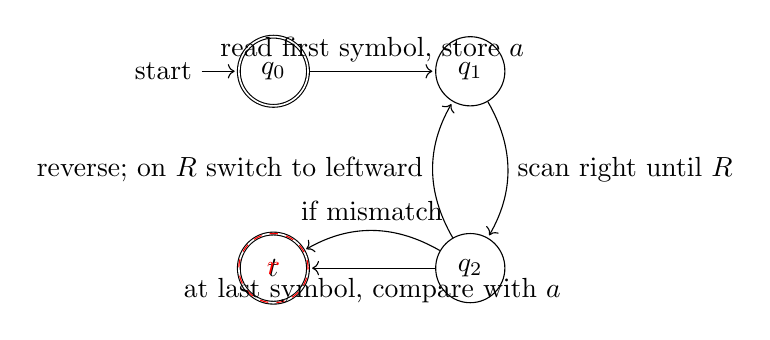
\begin{tikzpicture}[shorten >=1pt,node distance=2.5cm,on grid,auto]
  \node[state,initial,accepting] (q0) {\(q_0\)};
  \node[state] (q1) [right=of q0] {\(q_1\)};
  \node[state] (q2) [below=of q1] {\(q_2\)};
  \node[state,accepting] (t) [left=of q2] {\(t\)};
  \node[state,rejecting] (r) [below=of q0] {\(r\)};

  \path[->]
    (q0) edge node {read first symbol, store \(a\)} (q1)
    (q1) edge [bend left] node {scan right until \(R\)} (q2)
    (q2) edge [bend left] node {reverse; on \(R\) switch to leftward} (q1)
    (q2) edge node {at last symbol, compare with \(a\)} (t)
    (q2) edge [bend right] node [swap] {if mismatch} (r);
\end{tikzpicture}
\end{center}

\begin{figure}[h]
    \centering  
    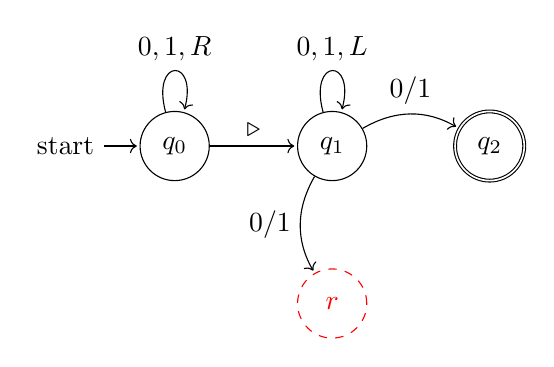
\begin{tikzpicture}[shorten >=1pt, node distance=2cm, on grid, auto]
        \node[state, initial] (q0) {\(q_0\)};
        \node[state] (q1) [right=of q0] {\(q_1\)};
        \node[state, accepting] (q2) [right=of q1] {\(q_2\)};
        \node[state, rejecting] (qr) [below=of q1] {\(r\)};
        \path[->]
            (q0) edge [loop above] node {\(0,1,R\)} (q0)
            (q0) edge node {\(\triangleright\)} (q1)
            (q1) edge [loop above] node {\(0,1,L\)} (q1)
            (q1) edge [bend left] node {\(0/1\)} (q2)
            (q1) edge [bend right] node[swap] {\(0/1\)} (qr);
    \end{tikzpicture}
    \caption{Schematic 2NFA illustrating a guess-and-check mechanism (for a toy symmetry language).}
    \label{fig:2nfa-example}
\end{figure}

\begin{figure}[h]
    \centering  
    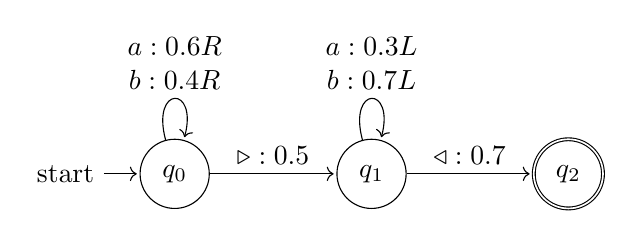
\begin{tikzpicture}[shorten >=1pt, node distance=2.5cm, on grid, auto]
        \node[state, initial] (q0) {\(q_0\)};
        \node[state] (q1) [right=of q0] {\(q_1\)};
        \node[state, accepting] (q2) [right=of q1] {\(q_2\)};
        \path[->]
            (q0) edge [loop above] node[align=center] {\(a:0.6R\)\\\(b:0.4R\)} (q0)
            (q0) edge node {\(\triangleright:0.5\)} (q1)
            (q1) edge [loop above] node[align=center] {\(a:0.3L\)\\\(b:0.7L\)} (q1)
            (q1) edge node {\(\triangleleft:0.7\)} (q2);
    \end{tikzpicture}
    \caption{Schematic 2PFA for a majority language (with sample probabilistic transitions).}
    \label{fig:2pfa-example}
\end{figure}


% \subsection{Key Theorems}
% \label{subsec:key-theorems} 

% \begin{enumerate}
%     \item \textit{Kleene's Theorem}: A language is regular if and only if it is recognized by a DFA/NFA or described by a regular expression \cite{hopcroft2006introduction}.
%     \item \textit{Subset Construction Theorem}: Every NFA can be converted to an equivalent DFA, with up to $2^n$ states \cite{hopcroft2006introduction}.
%     \item \textit{Myhill-Nerode Theorem}: Characterizes $\text{REG}$ via string indistinguishability, forming the basis for DFA minimization \cite{hopcroft2006introduction}.
%     \item \textit{Rabin's Theorem}: PFAs recognize stochastic languages, a strict superset of $\text{REG}$ \cite{rabin1963probabilistic}.
%     \item \textit{Sipser's Theorem}: 2PFAs recognize $\text{REG}$ in logarithmic space but require exponential time for non-regular languages \cite{sipser1980halting}.
% \end{enumerate} 

% These theorems collectively delineate the boundaries of classical finite automata, setting the stage for quantum extensions in subsequent chapters. 


\newpage
\section{Quantum Mechanics Foundations}
\label{sec:quantum-foundations}

This section establishes the quantum mechanical principles underpinning quantum automata theory, emphasizing mathematical formalism and conceptual distinctions from classical systems. The discussion focuses on foundational postulates and their computational implications.



\subsection{Qubits and Quantum States}
\label{subsec:qubits}

\begin{definition}[Qubit]
A \emph{\gls{qubit}} is the fundamental unit of quantum information. It is represented as a normalised vector in a two-dimensional complex Hilbert space,
\[
\mathcal{H} = \mathbb{C}^2.
\]
\end{definition}

\begin{notation}[Computational Basis]
The standard (computational) basis states for a qubit are defined as
\[
|0\rangle = \begin{pmatrix} 1 \\ 0 \end{pmatrix}, \quad |1\rangle = \begin{pmatrix} 0 \\ 1 \end{pmatrix}.
\]
\end{notation}

\begin{definition}[General Qubit State]
A general state of a \gls{qubit} is given by
\[
|\psi\rangle = \alpha|0\rangle + \beta|1\rangle, \quad \text{with } |\alpha|^2 + |\beta|^2 = 1,
\]
where \(\alpha,\beta \in \mathbb{C}\) are the \emph{probability amplitudes}.
\end{definition}

\begin{remark}
Global phase factors—i.e. multiplying the state by an overall phase \(e^{i\gamma}\)—do not affect the physical properties of the qubit.
\end{remark}

\begin{example}[Bloch Sphere Representation]
  Any pure state of a \gls{qubit} can be written in the form
  \[
  |\psi\rangle = \cos\frac{\theta}{2}|0\rangle + e^{i\phi}\sin\frac{\theta}{2}|1\rangle,
  \]
  with \(\theta \in [0,\pi]\) and \(\phi \in [0,2\pi)\). Figure~\ref{fig:bloch_sphere} illustrates the \textbf{Bloch sphere} representation of a qubit \cite{nielsen2010quantum}.
\end{example}

\begin{figure}[h]
  \centering
  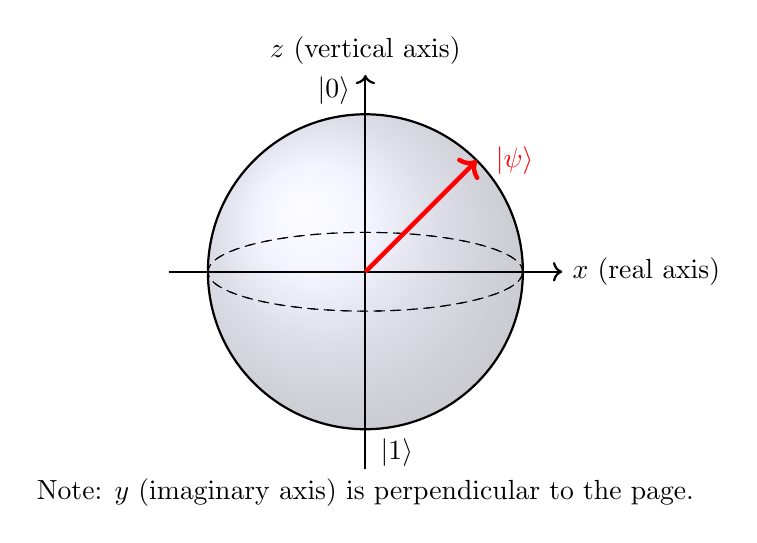
\begin{tikzpicture}[scale=1]
    % Draw sphere outline with shading
    \shade[ball color=blue!20, opacity=0.3] (0,0) circle (2cm);
    \draw[thick] (0,0) circle (2cm);
    
    % Draw equator as a dashed ellipse (horizontal cross-section)
    \draw[dashed] (0,0) ellipse (2cm and 0.5cm);
    
    % Draw meridian arcs (vertical cross-sections)
    \draw[dashed] (-2,0) arc (180:0:2cm and 0.5cm);
    \draw[dashed] (2,0) arc (0:-180:2cm and 0.5cm);
    
    % Axes: x and z
    \draw[->, thick] (-2.5,0) -- (2.5,0) node[right] {$x$ (real axis)};
    \draw[->, thick] (0,-2.5) -- (0,2.5) node[above] {$z$ (vertical axis)};
    
    % Mark north and south poles with horizontal shift
    \node[above, xshift=-0.4cm] at (0,2) {\(|0\rangle\)};
    \node[below, xshift=0.4cm] at (0,-2) {\(|1\rangle\)};
    
    % Bloch vector in the x-z plane
    \draw[->, red, ultra thick] (0,0) -- (1.414,1.414) node[right] {\(\;|\psi\rangle\)};
    
    % Note for y axis
    \node at (0,-2.8) {Note: \(y\) (imaginary axis) is perpendicular to the page.};
  \end{tikzpicture}
  \caption{Enhanced Bloch sphere representation of a \gls{qubit} with adjusted labels.}
  \label{fig:bloch_sphere}
  \end{figure}

\begin{observation}
  For multi-qubit systems, the overall state space is given by the tensor product of individual qubit spaces. For instance, a two-qubit system is described by
  \[
  |\psi\rangle = \sum_{i,j \in \{0,1\}} \alpha_{ij}\, |i\rangle \otimes |j\rangle, \quad \sum_{i,j} |\alpha_{ij}|^2 = 1.
  \]
  This exponential scaling of the state space underpins the potential of quantum parallelism \cite{nielsen2010quantum}.
\end{observation}



\subsection{Superposition and Entanglement}
\label{subsec:superposition}

\textbf{Superposition} enables parallel computation. The Hadamard gate ($H$) creates uniform superpositions:
\[
H|0\rangle = \frac{|0\rangle + |1\rangle}{\sqrt{2}}, \quad H|1\rangle = \frac{|0\rangle - |1\rangle}{\sqrt{2}}.
\]

\textbf{Entanglement} arises in multi-qubit states that cannot be factored. The Bell states are maximally entangled:
\[
|\Phi^+\rangle = \frac{|00\rangle + |11\rangle}{\sqrt{2}}, \quad |\Phi^-\rangle = \frac{|00\rangle - |11\rangle}{\sqrt{2}},
\]
\[
|\Psi^+\rangle = \frac{|01\rangle + |10\rangle}{\sqrt{2}}, \quad |\Psi^-\rangle = \frac{|01\rangle - |10\rangle}{\sqrt{2}}.
\]

\begin{figure}[h]
\centering
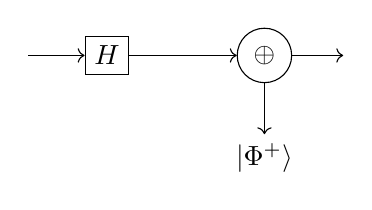
\begin{tikzpicture}
  \node[draw,rectangle] (h) at (0,0) {$H$};
  \node[draw,circle] (cnot) at (2,0) {$\oplus$};
  \draw[->] (-1,0) -- (h);
  \draw[->] (h) -- (cnot);
  \draw[->] (cnot) -- (3,0);
  \draw[->] (cnot) -- (2,-1) node[below] {$|\Phi^+\rangle$};
\end{tikzpicture}
\caption{Quantum circuit generating the Bell state $|\Phi^+\rangle$.}
\label{fig:bell_circuit}
\end{figure}

Entanglement is critical for quantum teleportation \cite{bennett1993teleporting} and enables exponential speedups in algorithms like Shor's \cite{shor1999polynomial}.

\subsection{Quantum Gates and Circuits}
\label{subsec:gates}

\begin{definition}[Quantum Gate]
A \emph{quantum gate} is a unitary operator \(U\) acting on a quantum state, meaning that \(U^\dagger U = I\). Quantum gates manipulate \glspl{qubit} and form the basic operations in quantum circuits.
\end{definition}

\begin{notation}[Single-Qubit Gates]
Key single-qubit gates include:
\begin{itemize}
    \item \textbf{Pauli-X (bit-flip):}
    \[
    X = \begin{pmatrix} 0 & 1 \\ 1 & 0 \end{pmatrix},
    \]
    which performs \(X|0\rangle = |1\rangle\) and \(X|1\rangle = |0\rangle\).
    \item \textbf{Hadamard:}
    \[
    H = \frac{1}{\sqrt{2}}\begin{pmatrix} 1 & 1 \\ 1 & -1 \end{pmatrix},
    \]
    creating superpositions as seen in the previous section.
    \item \textbf{Phase Shift:}
    \[
    R_\phi = \begin{pmatrix} 1 & 0 \\ 0 & e^{i\phi} \end{pmatrix}.
    \]
\end{itemize}
\end{notation}

\begin{definition}[Two-Qubit Gate]
A two-qubit gate, such as the \gls{cnot} gate, acts on a pair of qubits. The \gls{cnot} gate flips the second (target) qubit if the first (control) qubit is \(|1\rangle\); formally,
\[
\text{CNOT}|a\rangle|b\rangle = |a\rangle|a \oplus b\rangle,
\]
where \(\oplus\) denotes addition modulo 2.
\end{definition}

\begin{remark}
A universal set of quantum gates, for example \(\{H, T, \gls{cnot}\}\), can approximate any unitary operation to arbitrary precision, thereby forming the foundation of the quantum circuit model.
\end{remark}

\begin{example}[Deutsch-Jozsa Quantum Circuit]
Figure~\ref{fig:deutsch_circuit} shows a quantum circuit used in the Deutsch-Jozsa algorithm. The circuit demonstrates the application of Hadamard gates before and after the oracle \(U_f\), highlighting the interplay of superposition and entanglement in quantum computation.
\end{example}

\begin{figure}[h]
\centering
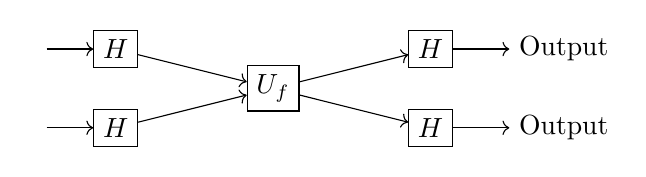
\begin{tikzpicture}[node distance=1.8cm, auto]
    \node (in1) at (0,0) {};
    \node (in2) at (0,-1) {};
    \node[draw, rectangle] (H1) at (1,0) {$H$};
    \node[draw, rectangle] (H2) at (1,-1) {$H$};
    \node[draw, rectangle] (Uf) at (3, -0.5) {\(U_f\)};
    \node[draw, rectangle] (H3) at (5,0) {$H$};
    \node[draw, rectangle] (H4) at (5,-1) {$H$};
    \draw[->] (in1) -- (H1);
    \draw[->] (in2) -- (H2);
    \draw[->] (H1) -- (Uf);
    \draw[->] (H2) -- (Uf);
    \draw[->] (Uf) -- (H3);
    \draw[->] (Uf) -- (H4);
    \draw[->] (H3) -- ++(1,0) node[right] {Output};
    \draw[->] (H4) -- ++(1,0) node[right] {Output};
\end{tikzpicture}
\caption{Quantum circuit for the Deutsch-Jozsa algorithm.}
\label{fig:deutsch_circuit}
\end{figure}

\subsection{Measurement and Probabilistic Outcomes}
\label{subsec:measurement}

Measurement in quantum mechanics is a fundamentally probabilistic process. When a quantum system in state
\[
|\psi\rangle = \sum_i \alpha_i|i\rangle
\]
is measured in the orthonormal basis \(\{|i\rangle\}\), the \textbf{Born rule} states that the outcome corresponding to \(|i\rangle\) is observed with probability
\[
P(i) = |\alpha_i|^2.
\]
This process is typically described as a \emph{projective measurement}, after which the state collapses to the observed eigenstate.

More generally, measurements can be described by \textbf{Positive Operator-Valued Measures (POVMs)}, which provide a framework for describing generalized measurements that are not necessarily projective. In a POVM, each measurement outcome is associated with a positive operator \(E_i\) satisfying \(\sum_i E_i = I\). The probability of outcome \(i\) is then given by
\[
P(i) = \langle\psi| E_i |\psi\rangle.
\]

For example, measuring the Bell state \( |\Phi^+\rangle = \frac{|00\rangle + |11\rangle}{\sqrt{2}} \) in the computational basis yields the outcomes \( |00\rangle \) or \( |11\rangle \) with 50\% probability each, as summarized in Table~\ref{tab:bell_measurement}.

\begin{table}[h]
\centering
\caption{Measurement outcomes for \( |\Phi^+\rangle \).}
\label{tab:bell_measurement}
\begin{tabular}{|c|c|}
\hline
\textbf{Outcome} & \textbf{Probability} \\ \hline
\( |00\rangle \)      & 50\%                \\ \hline
\( |11\rangle \)      & 50\%                \\ \hline
\end{tabular}
\end{table}

Measurement is an irreversible process and plays a critical role in quantum algorithms as well as in quantum automata theory, where it provides the means to extract classical information from quantum computations.

Mixed states, which describe statistical ensembles of quantum states, are represented by density matrices:
\[
\rho = \sum_i p_i |\psi_i\rangle\langle\psi_i|,
\]
with \(p_i \ge 0\) and \(\sum_i p_i = 1\). This formalism is essential when considering open systems subject to decoherence.


\subsection{Decoherence and Open Systems}
\label{subsec:decoherence}

\begin{definition}[Decoherence]
\emph{Decoherence} is the process by which a quantum system loses its coherent properties due to interaction with its environment. This results in the decay of the off-diagonal elements in the system's density matrix, leading the system to behave more classically.
\end{definition}

\begin{remark}
Decoherence is a major obstacle in quantum computing because it degrades the quantum correlations needed for quantum parallelism and entanglement.
\end{remark}

\begin{definition}[Lindblad Master Equation]
The evolution of an open quantum system can be described by the \textbf{Lindblad master equation}:
\[
\frac{d\rho}{dt} = -\frac{i}{\hbar}\,[H, \rho] + \sum_k \left( L_k \rho L_k^\dagger - \frac{1}{2}\{L_k^\dagger L_k, \rho\} \right),
\]
where \(\rho\) is the density matrix, \(H\) is the Hamiltonian, and \(L_k\) are the Lindblad (noise) operators \cite{breuer2002theory}.
\end{definition}

\begin{example}[Noise Models]
    Typical noise models include:
    \begin{itemize}
        \item \textbf{Amplitude damping}: Models energy loss (e.g., spontaneous emission) \cite{nielsen2010quantum}.
        \item \textbf{Phase damping}: Represents the loss of phase coherence without energy dissipation \cite{nielsen2010quantum}.
    \end{itemize}
\end{example}

\begin{observation}
    To combat decoherence, quantum error correction codes (such as the Shor code \cite{shor1995scheme} and surface codes \cite{fowler2012surface}) and decoherence-free subspaces are employed.
\end{observation}
 

\chapter{Literature Review}
\label{chap:chapter3}

\section{One-way QFAs}
\label{sec:one-way-qfas}

\subsection{Standard Models}
\label{subsec:standard-models}

\subsubsection{MO-1QFA (Measure-Once)}
\label{sssec:mo-1qfa}

\textbf{Definition}: An MO-1QFA is defined as \( M = (Q, \Sigma, \delta, q_0, F) \), where:
- \( Q \): Finite set of quantum basis states.
- \( \Sigma \): Input alphabet with end-marker \( \# \).
- \( \delta \): Transition function inducing unitary operators \( U_\sigma \) for \( \sigma \in \Sigma \).
- \( q_0 \in Q \): Initial state.
- \( F \subseteq Q \): Accepting states \cite{moore2000quantum}.

\textbf{Operation}: Processes input sequentially with a single measurement at the end. The state evolves as \( |\psi_i\rangle = U_{\sigma_i}|\psi_{i-1}\rangle \). Acceptance is determined by projecting onto \( F \) \cite{moore2000quantum}.

\textbf{Key Features}:
- Recognizes a strict subset of regular languages (e.g., periodic languages) \cite{bertoni2001regular}.
- Requires \( O(n) \) states for languages like \( L_{\text{mod}} = \{w \mid |w| \equiv 0 \mod p\} \).

\textbf{Limitations}: 
- Cannot recognize non-regular languages like \( L_{\text{eq}} = \{a^n b^n\} \).

\subsubsection{MM-1QFA (Measure-Many)}
\label{sssec:mm-1qfa}

\textbf{Definition}: An MM-1QFA is \( M = (Q, \Sigma, \delta, q_0, Q_{\text{acc}}, Q_{\text{rej}}, Q_{\text{non}}) \), where:
- \( Q_{\text{acc}}, Q_{\text{rej}}, Q_{\text{non}} \): Partitioned states for halting and continuation \cite{kondacs1997power}.

\textbf{Operation}: Measures after each symbol, halting if \( Q_{\text{acc}} \) or \( Q_{\text{rej}} \) is observed \cite{kondacs1997power}.

\textbf{Key Features}:
- Recognizes non-regular languages (e.g., \( L_{\text{eq}} \)) with bounded error \cite{kondacs1997power}.
- Exponential state advantage over DFAs for certain languages \cite{ambainis2009superiority}.

\textbf{Limitations}: 
- Strictly less powerful than two-way QFAs \cite{ambainis2009superiority}.

\subsubsection{LQFA (Latvian)}
\label{sssec:lqfa}

\textbf{Definition}: Combines unitary operations and projective measurements. Defined as \( M = (Q, \Sigma, \delta, q_0, F) \), where transitions include measurements \cite{ambainis2002quantum}.

\textbf{Operation}: Applies unitary transformations followed by projective measurements at each step \cite{ambainis2002quantum}.

\textbf{Key Features}:
- Recognizes a proper subset of MM-1QFA languages \cite{ambainis2002quantum}.
- Fails to recognize regular languages like \( a\Sigma^* \).

\textbf{Limitations}: 
- Weaker closure properties compared to MM-1QFA \cite{ambainis2002quantum}.

\subsection{Hybrid Models}
\label{subsec:hybrid-models}

\subsubsection{1QFAC (Classical States)}
\label{sssec:1qfac}

\textbf{Definition}: \( M = (S, Q, \Sigma, \delta, \mu, s_0, q_0, F) \), combining classical control \( S \) and quantum states \( Q \) \cite{zheng2012one}.

\textbf{Operation}: Classical state \( s_i \) selects quantum operator \( \mu(s_i, \sigma) \). Measurement occurs only at the end \cite{zheng2012one}.

\textbf{Key Features}:
- Recognizes all regular languages and some non-regular languages (e.g., \( L_{\text{eq}} \)) \cite{zheng2012one}.
- Exponentially more succinct than DFAs for certain languages \cite{bianchi2014size}.

\textbf{Limitations}: 
- Requires careful error correction due to quantum-classical interaction \cite{zheng2012one}.

\subsubsection{CL-1QFA (Control Languages)}
\label{sssec:cl-1qfa}

\textbf{Definition}: Uses control languages to guide measurements. Defined as \( M = (Q, \Sigma, \delta, q_0, \mathcal{L}) \), where \( \mathcal{L} \) specifies allowed measurement outcomes \cite{bertoni2003quantum}.

\textbf{Operation}: Applies unitary operations and projects onto subspaces dictated by \( \mathcal{L} \) \cite{bertoni2003quantum}.

\textbf{Key Features}:
- Closed under Boolean operations \cite{bertoni2003quantum}.
- Recognizes regular languages with bounded error \cite{bertoni2003quantum}.

\textbf{Limitations}: 
- Complex control logic increases implementation overhead \cite{bertoni2003quantum}.

\subsection{Enhanced Models}
\label{subsec:enhanced-models}

\subsubsection{EQFA (Enhanced)}
\label{sssec:eqfa}

\textbf{Definition}: Uses ancilla qubits and arbitrary measurements. Defined as \( M = (\Sigma, Q, \{U_\sigma\}, Q_{\text{acc}}, Q_{\text{rej}}, Q_{\text{non}}, q_0) \) \cite{paschen2000quantum}.

\textbf{Operation}: Employs mixed states and non-unitary transitions for enhanced expressiveness \cite{paschen2000quantum}.

\textbf{Key Features}:
- Simulates all classical finite automata \cite{paschen2000quantum}.
- Recognizes non-regular languages with unbounded error \cite{nayak1999optimal}.

\textbf{Limitations}: 
- Irreversible operations complicate error analysis \cite{nayak1999optimal}.

\subsubsection{OT-QFA (Open-Time Evolution)}
\label{sssec:ot-qfa}

\textbf{Definition}: Incorporates environmental noise via Lindblad dynamics. Defined as \( M = (\Sigma, Q, \mathcal{L}, q_0, F) \), where \( \mathcal{L} \) models decoherence \cite{hirvensalo2012quantum}.

\textbf{Operation}: State evolution governed by the Lindblad equation, with measurement at the end \cite{hirvensalo2012quantum}.

\textbf{Key Features}:
- Generalizes MO-1QFA and MM-1QFA \cite{hirvensalo2012quantum}.
- Models realistic noisy systems \cite{breuer2002theory}.

\textbf{Limitations}: 
- Undecidable properties due to open-system dynamics \cite{hirvensalo2012quantum}.

\subsubsection{A-QFA (Ancilla-Based)}
\label{sssec:a-qfa}

\textbf{Definition}: Extends MO-1QFA with ancilla qubits. Defined as \( M = (Q, \Sigma, \delta, q_0, F) \) with an expanded Hilbert space \cite{paschen2000quantum}.

\textbf{Operation}: Uses ancillae to simulate classical nondeterminism via quantum interference \cite{paschen2000quantum}.

\textbf{Key Features}:
- Recognizes all regular languages with certainty \cite{paschen2000quantum}.
- Handles non-regular languages with one-sided error \cite{paschen2000quantum}.

\textbf{Limitations}: 
- Ancilla management increases resource overhead \cite{paschen2000quantum}.

\subsection{Advanced Variants}
\label{subsec:advanced-variants}

\subsubsection{1.5QFA (1.5-Way)}
\label{sssec:1.5qfa}

\textbf{Definition}: Allows limited head movement. Defined as \( M = (Q, \Sigma, \delta, q_0, F) \), where \( \delta \) restricts leftward motion \cite{kondacs1997power}.

\textbf{Operation}: Head moves right or remains stationary but cannot backtrack fully \cite{kondacs1997power}.

\textbf{Key Features}:
- Recognizes non-regular languages with bounded error \cite{kondacs1997power}.
- Strictly more powerful than MO-1QFA \cite{kondacs1997power}.

\textbf{Limitations}: 
- Less powerful than 2QFA \cite{kondacs1997power}.

\subsubsection{ML-QFA (Multi-Letter)}
\label{sssec:ml-qfa}

\textbf{Definition}: Reads \( k \)-symbol blocks. Defined as \( M = (Q, \Sigma, \delta, q_0, F) \), where \( \delta \) depends on \( k \)-length substrings \cite{belovs2007multi}.

\textbf{Operation}: Processes input in chunks, applying unitary operators for each block \cite{belovs2007multi}.

\textbf{Key Features}:
- Simulates multi-head classical automata \cite{belovs2007multi}.
- Recognizes context-sensitive languages with bounded error \cite{belovs2007multi}.

\textbf{Limitations}: 
- State complexity grows exponentially with \( k \) \cite{belovs2007multi}.
% \chapter{Literature Review}
% \label{chap:chapter3}
% \section{One-way QFAs}
% \subsection{Standard Models}
% \subsubsection{MO-1QFA (Measure-Once)}
% \subsubsection{MM-1QFA (Measure-Many)}
% \subsubsection{LQFA (Latvian)}
% \subsection{Hybrid Models}
% \subsubsection{1QFAC (Classical States)}
% \subsubsection{CL-1QFA (Control Languages)}
% \subsection{Enhanced Models}
% \subsubsection{EQFA (Enhanced)}
% \subsubsection{OT-QFA (Open-Time Evolution)}
% \subsubsection{A-QFA (Ancilla-Based)}
% \subsection{Advanced Variants}
% \subsubsection{1.5QFA (1.5-Way)}
% \subsubsection{ML-QFA (Multi-Letter)}

\section{Two-way QFAs}
\label{sec:two-way-qfas}

\subsection{Standard Models}
\label{subsec:two-way-standard}

\subsubsection{2QFA (Two-Way)}
\label{sssec:2qfa}

\textbf{Definition}: A 2QFA is defined as \( M = (Q, \Sigma, \delta, q_0, Q_{\text{acc}}, Q_{\text{rej}}) \), where:
- \( Q \): Finite set of quantum states partitioned into \( Q_{\text{acc}} \), \( Q_{\text{rej}} \), and \( Q_{\text{non}} \).
- \( \Sigma \): Input alphabet with end-markers \( \# \) (left) and \( \$ \) (right).
- \( \delta \): Transition function defining unitary operators and head movements \( \{ \leftarrow, \rightarrow, \downarrow \} \) \cite{kondacs1997power}.

\textbf{Operation}: The head moves bidirectionally over the input tape. For input \( w = \sigma_1\sigma_2\ldots\sigma_n \), the state evolves as \( |\psi_i\rangle = U_{\sigma_i} |\psi_{i-1}\rangle \), with intermediate measurements allowed \cite{kondacs1997power}.

\textbf{Key Features}:
- Recognizes non-regular languages (e.g., \( L_{\text{eq}} = \{a^n b^n\} \)) with bounded error in linear time \cite{kondacs1997power}.
- Solves the word problem for finitely generated groups \cite{ambainis2002quantum}.

\textbf{Limitations}: 
- Requires quantum registers scaling with input length, complicating physical implementation \cite{ambainis2002quantum}.

\subsection{Hybrid Models}
\label{subsec:two-way-hybrid}

\subsubsection{2QCFA (Classical States)}
\label{sssec:2qcfa}

\textbf{Definition}: Combines classical control and quantum states. Defined as \( M = (S, Q, \Sigma, \Theta, \delta, s_0, q_0, S_{\text{acc}}, S_{\text{rej}}) \), where:
- \( S \): Classical states controlling transitions.
- \( Q \): Quantum states for superposition/mixed states \cite{ambainis2002quantum}.

\textbf{Operation}: Classical states \( S \) select quantum operations \( \Theta \), while \( \delta \) governs head movement. Measurements occur adaptively based on classical control \cite{ambainis2002quantum}.

\textbf{Key Features}:
- Recognizes \( L_{\text{eq}} \) and palindromes \( L_{\text{pal}} = \{ww^R\} \) in polynomial time with constant quantum states \cite{ambainis2002quantum}.
- Simulates classical 2PFAs while recognizing non-regular languages \cite{zheng2012one}.

\textbf{Limitations}: 
- Decidability of equivalence between 2QCFAs remains open \cite{zheng2012one}.

\subsection{Multihead/Tape Extensions}
\label{subsec:multihead-tape}

\subsubsection{2TQCFA (Two-Tape)}
\label{sssec:2tqcfa}

\textbf{Definition}: Extends 2QCFA with two tapes. Defined as \( M = (S, Q, \Sigma_1 \times \Sigma_2, \Theta, \delta, s_0, q_0, S_{\text{acc}}, S_{\text{rej}}) \), where:
- \( \Sigma_1, \Sigma_2 \): Input alphabets for two tapes.
- \( \delta \): Governs synchronized head movements on both tapes \cite{zheng2012two}.

\textbf{Operation}: Processes inputs on two tapes simultaneously, enabling verification of relationships like \( L = \{a^n b^n c^n\} \) \cite{zheng2012two}.

\textbf{Key Features}:
- Recognizes languages beyond the capabilities of single-tape 2QFAs \cite{zheng2012two}.
- Verifies non-context-free languages in polynomial time \cite{zheng2012two}.

\textbf{Limitations}: 
- Increased complexity in synchronization and error correction \cite{zheng2012two}.

\subsubsection{kTQCFA (k-Tape)}
\label{sssec:ktqcfa}

\textbf{Definition}: Generalizes 2TQCFA to \( k \) tapes. Defined as \( M = (S, Q, \bigtimes_{i=1}^k \Sigma_i, \Theta, \delta, s_0, q_0, S_{\text{acc}}, S_{\text{rej}}) \) \cite{zheng2012two}.

\textbf{Operation}: Coordinates \( k \) independent tapes for parallel processing, useful for multi-variable language recognition \cite{zheng2012two}.

\textbf{Key Features}:
- Recognizes \( L = \{a^n b^{n^2}\} \) with \( O(\log n) \) quantum states \cite{zheng2012two}.
- Subsumes classical multi-tape automata in efficiency \cite{zheng2012two}.

\textbf{Limitations}: 
- Practical implementation constrained by tape synchronization overhead \cite{zheng2012two}.

% \section{Two-way QFAs}
% \subsection{Standard Models}
% \subsubsection{2QFA (Two-Way)}
% \subsection{Hybrid Models}
% \subsubsection{2QCFA (Classical States)}
% \subsection{Multihead/Tape Extensions}
% \subsubsection{2TQCFA (Two-Tape)}
% \subsubsection{kTQCFA (k-Tape)}

\section{Interactive Quantum Automata}
\label{sec:interactive-quantum}

\subsubsection{QIP (Quantum Interactive Proofs)}
\label{sssec:qip}

\textbf{Definition}: A \textit{Quantum Interactive Proof} (QIP) system involves a polynomial-time quantum verifier \( V \) interacting with an unbounded quantum prover \( P \) via a shared quantum channel. The verifier is modeled as a quantum finite automaton (QFA) with limited memory \cite{zheng2015power}. Formally, \( \text{QIP}(k) \) denotes systems with \( k \) rounds of interaction \cite{nishimura2009application}.

\textbf{Operation}: The verifier processes input \( w \) through alternating rounds of quantum communication with the prover. For 1QFA/2QFA verifiers, transitions are governed by:
\[
\delta: Q \times \Sigma \times \Gamma \to \mathbb{C}^{Q \times Q},
\]
where \( \Gamma \) is the communication alphabet \cite{zheng2015power}. Acceptance is determined by measuring the verifier's final state.

\textbf{Key Features}:
- \( \text{QIP} = \text{PSPACE} \) [[1], [2]], demonstrating equivalence to classical interactive proofs.
- QFA-based verifiers (e.g., 2QFA) recognize languages beyond regular classes with bounded error \cite{nishimura2009application}.
- Two-message QIP systems (\( \text{QIP}(2) \)) are contained in \( \text{PSPACE} \) <button class="citation-flag" data-index="1">.

\textbf{Limitations}: 
- Requires precise control over quantum communication channels \cite{zheng2015power}.
- Verifier's state complexity scales with input length for non-regular languages \cite{nishimura2009application}.

\subsubsection{QMIP (Quantum Merlin-Arthur)}
\label{sssec:qmip}

\textbf{Definition}: \textit{Quantum Merlin-Arthur} (QMIP) extends QIP to multiple quantum provers (\( k \geq 2 \)) who cannot communicate. Defined as \( \text{QMIP}(k) \), it allows entangled provers but restricts collusion \cite{scegulnaja2010postselection}.

\textbf{Operation}: Merlin (prover) sends a quantum witness state \( |\psi\rangle \) to Arthur (verifier). For 2QFA verifiers, the transition function validates \( |\psi\rangle \) via:
\[
\delta: Q \times \Sigma \times \mathcal{H}_\text{wit} \to \mathbb{C}^{Q \times Q},
\]
where \( \mathcal{H}_\text{wit} \) is the witness Hilbert space \cite{yamakami2014constant}.

\textbf{Key Features}:
- \( \text{QMIP} = \text{MIP}^* \), enabling recognition of languages beyond \( \text{QIP} \) <button class="citation-flag" data-index="10">.
- Recognizes the palindrome language \( L_{\text{pal}} = \{ww^R\} \) with entangled provers \cite{scegulnaja2010postselection}.
- 2QFA verifiers with QMIP achieve exponential state savings over classical MIP systems \cite{zheng2015power}.

\textbf{Limitations}: 
- Entanglement between provers introduces verification complexity \cite{yamakami2014constant}.
- \( \text{QMIP}(1\text{QFA}) \neq \text{QIP}(1\text{QFA}) \) in polynomial time \cite{nishimura2009application}.

% \section{Interactive Quantum Automata}
% \subsubsection{QIP (Quantum Interactive Proofs)}
% \subsubsection{QMIP (Quantum Merlin-Arthur)}

\chapter{Comparative Analysis}
\label{chap:comparative-analysis}

The literature on \gls{qfa} reveals a diverse landscape of computational models, each tailored to balance quantum resources with expressive power. At the most fundamental level, one-way \glspl{qfa} such as MO-1QFA and MM-1QFA offer elegant, conceptually simple frameworks. For instance, the MO-1QFA model—employing a single measurement at the end—boasts straightforward dynamics that, however, limit its language recognition capabilities to reversible regular languages. In contrast, the MM-1QFA interweaves unitary evolution with intermediate measurements, thereby extending its acceptance range to include a larger subset of regular languages and, in some cases, even non-regular languages under bounded error conditions. This increase in expressive power, however, is not without cost; the integration of frequent measurements adds complexity in terms of error management and circuit design.

Hybrid models, such as 1QFAC and CL-1QFA, seek to blend classical control mechanisms with quantum processing. The 1QFAC model, for example, leverages classical state control to effectively simulate deterministic finite automata, thereby recognizing all regular languages and sometimes even certain non-regular languages with significant state savings. Meanwhile, the CL-1QFA employs control languages that guide the measurement outcomes, ensuring desirable closure properties under Boolean operations. These models illustrate a recurring theme: as expressive power increases, so does the need for intricate coordination between quantum and classical elements.

Enhanced models push these boundaries further. EQFA and OT-QFA introduce non-unitary evolution through superoperators or completely positive trace-preserving (CPTP) maps, which not only enable the simulation of classical automata but also, in some cases, facilitate the recognition of non-regular languages. Similarly, the A-QFA model uses ancilla qubits to simulate additional quantum resources, providing a pathway to overcome the inherent limitations of simpler QFA models. However, the richer dynamics offered by these enhanced models come at the price of increased resource requirements and greater susceptibility to decoherence and noise.

Turning to two-way QFAs, models such as 2QFA and 2QCFA leverage bidirectional head movement to harness quantum interference more effectively. The 2QFA, with its unrestricted movement, can recognize certain non-regular languages (e.g., \( \{a^n b^n\} \)) in linear time under bounded error, yet it demands quantum registers that grow with the input size. On the other hand, the hybrid 2QCFA mitigates some of this cost by integrating classical control with a small quantum register. This trade-off allows 2QCFA to recognize complex languages—such as palindromes—using only a constant number of quantum states, albeit at the expense of a more complicated synchronization mechanism between the classical and quantum components.

Multihead and multitape extensions, exemplified by 2TQCFA and kTQCFA, further amplify computational power by enabling parallel processing across multiple input streams. These models are particularly effective for languages characterized by intricate structural dependencies. While they offer substantial gains in expressiveness, their increased complexity in synchronizing multiple tape heads and managing error correction represents a significant engineering challenge.

Interactive models, encompassing QIP and QMIP systems, introduce an additional layer of computational interplay. QIP systems couple a resource-limited quantum verifier with a single unbounded prover, thereby linking QFA models to complexity classes such as PSPACE. QMIP systems extend this framework to incorporate multiple non-communicating provers, a development that not only increases verification power but also opens the door to recognizing languages beyond the reach of single-prover systems. The practical implementation of such systems, however, is complicated by the need to manage quantum entanglement and the inherent sensitivity of the communication channels.

\vspace{0.5em}
In summary, the spectrum of QFA models represents a delicate balance: simpler one-way models achieve low resource overhead at the expense of expressive power, while hybrid, enhanced, two-way, and interactive models incrementally increase language recognition capabilities—albeit with concomitant increases in state complexity, error management demands, and implementation challenges.

%%%%%%%%%%%%%%%%%%%%%%%%%%%%%%%%%%%%%%%%%%%%%%%%%%%%%%%%%%%%%%
\subsection*{Schematic Comparative Overview}

\begin{table}[ht]
\centering
\begin{tabular}{|l|l|l|}
\hline
\textbf{Model Category} & \textbf{Expressive Power (Languages Accepted)} & \textbf{Resource/Cost Trade-offs} \\
\hline
One-way QFAs & \begin{tabular}[c]{@{}l@{}}MO-1QFA: Reversible regular\\ MM-1QFA: Larger subset of regular (+some non-regular)\\ LQFA: Trade-off between measurement overhead and expressiveness\end{tabular} 
& Low complexity, limited expressive power; intermediate measurements increase design overhead \\
\hline
Hybrid Models & \begin{tabular}[c]{@{}l@{}}1QFAC: All regular (sometimes non-regular)\\ CL-1QFA: Enhanced closure properties\end{tabular} 
& Integration of classical control reduces quantum state requirements; additional coordination complexity \\
\hline
Enhanced Models & \begin{tabular}[c]{@{}l@{}}EQFA/OT-QFA: Simulate classical automata, recognize some non-regular languages\\ A-QFA: Additional quantum resources via ancilla qubits\end{tabular} 
& Non-unitary operations and open system dynamics incur higher resource and error management costs \\
\hline
Two-way QFAs & \begin{tabular}[c]{@{}l@{}}2QFA: Some non-regular languages (e.g., \( \{a^n b^n\} \))\\ 2QCFA: Complex languages with constant quantum state usage\end{tabular} 
& Bidirectional motion enhances recognition but may require scaling quantum registers; synchronization challenges \\
\hline
Multihead/Tape Extensions & \begin{tabular}[c]{@{}l@{}}2TQCFA/kTQCFA: Languages with intricate dependencies\end{tabular} 
& Increased synchronization and parallel processing overhead \\
\hline
Interactive Models & \begin{tabular}[c]{@{}l@{}}QIP: Bounded-error languages (linked to PSPACE)\\ QMIP: Languages beyond single-prover capabilities (e.g., \( L_{\text{pal}} \))\end{tabular} 
& Complex communication protocols; high sensitivity to noise and decoherence \\
\hline
\end{tabular}
\caption{Comparative overview of QFA models in terms of expressive power and resource trade-offs.}
\label{tab:comparison}
\end{table}

%%%%%%%%%%%%%%%%%%%%%%%%%%%%%%%%%%%%%%%%%%%%%%%%%%%%%%%%%%%%%%
\subsection*{Graphical Comparison of QFA Models}
\begin{figure}[ht]
\centering
\begin{tikzpicture}[node distance=1.8cm, auto, every node/.style={draw, rectangle, align=center, minimum width=3cm, minimum height=1cm, font=\small}]
    % One-way models
    \node (MO1) {MO-1QFA};
    \node (MM1) [right=of MO1] {MM-1QFA};
    \node (LQFA) [right=of MM1] {LQFA};

    % Hybrid models below one-way
    \node (1QFAC) [below=of MO1] {1QFAC};
    \node (CL1) [below=of MM1] {CL-1QFA};

    % Enhanced models
    \node (EQFA) [below=of LQFA] {EQFA/OT-QFA};
    \node (AQFA) [right=of EQFA] {A-QFA};

    % Two-way models (top row)
    \node (2QFA) [above=of MO1] {2QFA};
    \node (2QCFA) [above=of MM1] {2QCFA};

    % Multihead/Tape
    \node (2TQCFA) [above=of 2QCFA, xshift=-1cm] {2TQCFA};
    \node (kTQCFA) [above=of 2QCFA, xshift=1cm] {kTQCFA};

    % Interactive models (separate branch)
    \node (QIP) [below=of AQFA, yshift=-1cm] {QIP};
    \node (QMIP) [right=of QIP] {QMIP};

    % Arrows indicating extension/increased expressive power
    \draw[->, thick] (MO1) -- (MM1);
    \draw[->, thick] (MM1) -- (LQFA);
    \draw[->, thick] (1QFAC) -- (CL1);
    \draw[->, thick] (2QFA) -- (2QCFA);
    \draw[->, thick] (2QCFA) -- (2TQCFA);
    \draw[->, thick] (2QCFA) -- (kTQCFA);
    \draw[->, thick] (QIP) -- (QMIP);
\end{tikzpicture}
\caption{Graphical comparison of QFA models. Horizontal and vertical arrows indicate extensions in expressive power and additional resource requirements. Models higher in the diagram are generally more expressive, while interactive models form an orthogonal extension capturing advanced computational paradigms.}
\label{fig:qfa-graphical}
\end{figure}

%%%%%%%%%%%%%%%%%%%%%%%%%%%%%%%%%%%%%%%%%%%%%%%%%%%%%%%%%%%%%%
\subsection*{Summary of Promising Models for Future Research}
Among the diverse models examined, the hybrid 2QCFA and the interactive QMIP systems appear particularly promising for future developments. The 2QCFA, by combining robust classical control with a minimal quantum component, offer an attractive balance between expressive power and practical resource constraints. Similarly, QMIP systems, despite their inherent complexity, pave the way for leveraging multiprover interactions to tackle verification problems beyond the reach of traditional single-prover systems.

Overall, this taxonomy not only reconciles previous inconsistencies in QFA definitions and capabilities but also provides a clear roadmap for exploring new frontiers in quantum automata theory. As quantum hardware matures, these models will be instrumental in designing efficient quantum algorithms and automata implementations that fully harness the potential of quantum computing.

\chapter{Conclusion}
\label{chap:chapter4}

 


\printglossary[title={Abbreviations},type=acronym,style=long]
\appendix
\printbibliography

\printindex

\chapter*{Acknowledgments}

Above all, this journey has been immensely rewarding, even though it was demanding and at times exhausting.

Since I began my studies at the University of Camerino, Michele Loreti has remained a steady mentor, and I am deeply grateful for his guidance.

I also value Marcello Bonsangue's generosity, openness, constant good humour, and sharp feedback.

Thank you to the LIACS staff and PhD students for creating a friendly and engaging environment. You made every day interesting and enjoyable, from lively whiteboard sessions to endless coffee breaks.

To my family: thank you for your steady support and for always being there. Mum, you have been my unfailing reference in all matters, ready with practical advice and help whenever I needed it.

To my friends in Camerino: thank you for turning that small town into the centre of the universe. A special shout-out to Alice, my anchor during the toughest moments.

Valentijn, thank you for making my time in the Netherlands even lovelier and for giving me a sense of home there. You stood by me during those life-changing months, bringing peace and calm when I needed them most.

I'm grateful to everyone I've met. Whether you encouraged me or pushed me, you influenced who I am today.

Lastly, I want to thank the version of me who set out on this adventure three years ago. Even without a clear destination, you kept your energy, curiosity, and resolve. I'm proud of who you've become; it was hard, but it was worth it.

\end{document}